\documentclass[twoside]{book}

% Packages required by doxygen
\usepackage{calc}
\usepackage{doxygen}
\usepackage{graphicx}
\usepackage[utf8]{inputenc}
\usepackage{makeidx}
\usepackage{multicol}
\usepackage{multirow}
\usepackage{textcomp}
\usepackage[table]{xcolor}

% Font selection
\usepackage[T1]{fontenc}
\usepackage{mathptmx}
\usepackage[scaled=.90]{helvet}
\usepackage{courier}
\usepackage{amssymb}
\usepackage{sectsty}
\renewcommand{\familydefault}{\sfdefault}
\allsectionsfont{%
  \fontseries{bc}\selectfont%
  \color{darkgray}%
}
\renewcommand{\DoxyLabelFont}{%
  \fontseries{bc}\selectfont%
  \color{darkgray}%
}

% Page & text layout
\usepackage{geometry}
\geometry{%
  a4paper,%
  top=2.5cm,%
  bottom=2.5cm,%
  left=2.5cm,%
  right=2.5cm%
}
\tolerance=750
\hfuzz=15pt
\hbadness=750
\setlength{\emergencystretch}{15pt}
\setlength{\parindent}{0cm}
\setlength{\parskip}{0.2cm}
\makeatletter
\renewcommand{\paragraph}{%
  \@startsection{paragraph}{4}{0ex}{-1.0ex}{1.0ex}{%
    \normalfont\normalsize\bfseries\SS@parafont%
  }%
}
\renewcommand{\subparagraph}{%
  \@startsection{subparagraph}{5}{0ex}{-1.0ex}{1.0ex}{%
    \normalfont\normalsize\bfseries\SS@subparafont%
  }%
}
\makeatother

% Headers & footers
\usepackage{fancyhdr}
\pagestyle{fancyplain}
\fancyhead[LE]{\fancyplain{}{\bfseries\thepage}}
\fancyhead[CE]{\fancyplain{}{}}
\fancyhead[RE]{\fancyplain{}{\bfseries\leftmark}}
\fancyhead[LO]{\fancyplain{}{\bfseries\rightmark}}
\fancyhead[CO]{\fancyplain{}{}}
\fancyhead[RO]{\fancyplain{}{\bfseries\thepage}}
\fancyfoot[LE]{\fancyplain{}{}}
\fancyfoot[CE]{\fancyplain{}{}}
\fancyfoot[RE]{\fancyplain{}{\bfseries\scriptsize Generated on Tue Mar 13 2018 22\-:09\-:49 for imachine by Doxygen }}
\fancyfoot[LO]{\fancyplain{}{\bfseries\scriptsize Generated on Tue Mar 13 2018 22\-:09\-:49 for imachine by Doxygen }}
\fancyfoot[CO]{\fancyplain{}{}}
\fancyfoot[RO]{\fancyplain{}{}}
\renewcommand{\footrulewidth}{0.4pt}
\renewcommand{\chaptermark}[1]{%
  \markboth{#1}{}%
}
\renewcommand{\sectionmark}[1]{%
  \markright{\thesection\ #1}%
}

% Indices & bibliography
\usepackage{natbib}
\usepackage[titles]{tocloft}
\setcounter{tocdepth}{3}
\setcounter{secnumdepth}{5}
\makeindex

% Hyperlinks (required, but should be loaded last)
\usepackage{ifpdf}
\ifpdf
  \usepackage[pdftex,pagebackref=true]{hyperref}
\else
  \usepackage[ps2pdf,pagebackref=true]{hyperref}
\fi
\hypersetup{%
  colorlinks=true,%
  linkcolor=blue,%
  citecolor=blue,%
  unicode%
}

% Custom commands
\newcommand{\clearemptydoublepage}{%
  \newpage{\pagestyle{empty}\cleardoublepage}%
}


%===== C O N T E N T S =====

\begin{document}

% Titlepage & ToC
\hypersetup{pageanchor=false}
\pagenumbering{roman}
\begin{titlepage}
\vspace*{7cm}
\begin{center}%
{\Large imachine }\\
\vspace*{1cm}
{\large Generated by Doxygen 1.8.6}\\
\vspace*{0.5cm}
{\small Tue Mar 13 2018 22:09:49}\\
\end{center}
\end{titlepage}
\clearemptydoublepage
\tableofcontents
\clearemptydoublepage
\pagenumbering{arabic}
\hypersetup{pageanchor=true}

%--- Begin generated contents ---
\chapter{Hierarchical Index}
\section{Class Hierarchy}
This inheritance list is sorted roughly, but not completely, alphabetically\-:\begin{DoxyCompactList}
\item \contentsline{section}{com\-:\-:ygomi\-:\-:roaddb\-:\-:util\-:\-:Abstract\-Dispatcher}{\pageref{classcom_1_1ygomi_1_1roaddb_1_1util_1_1AbstractDispatcher}}{}
\item \contentsline{section}{com\-:\-:ygomi\-:\-:roaddb\-:\-:util\-:\-:Message}{\pageref{classcom_1_1ygomi_1_1roaddb_1_1util_1_1Message}}{}
\item \contentsline{section}{com\-:\-:ygomi\-:\-:roaddb\-:\-:util\-:\-:Runnable}{\pageref{classcom_1_1ygomi_1_1roaddb_1_1util_1_1Runnable}}{}
\begin{DoxyCompactList}
\item \contentsline{section}{com\-:\-:ygomi\-:\-:roaddb\-:\-:util\-:\-:Work}{\pageref{classcom_1_1ygomi_1_1roaddb_1_1util_1_1Work}}{}
\end{DoxyCompactList}
\item \contentsline{section}{com\-:\-:ygomi\-:\-:roaddb\-:\-:util\-:\-:Thread\-Pool}{\pageref{classcom_1_1ygomi_1_1roaddb_1_1util_1_1ThreadPool}}{}
\item \contentsline{section}{com\-:\-:ygomi\-:\-:roaddb\-:\-:util\-:\-:T\-S\-Queue$<$ T $>$}{\pageref{classcom_1_1ygomi_1_1roaddb_1_1util_1_1TSQueue}}{}
\item \contentsline{section}{com\-:\-:ygomi\-:\-:roaddb\-:\-:util\-:\-:T\-S\-Queue$<$ com\-:\-:ygomi\-:\-:roaddb\-:\-:util\-:\-:Message $>$}{\pageref{classcom_1_1ygomi_1_1roaddb_1_1util_1_1TSQueue}}{}
\item \contentsline{section}{com\-:\-:ygomi\-:\-:roaddb\-:\-:util\-:\-:Work\-Thread}{\pageref{classcom_1_1ygomi_1_1roaddb_1_1util_1_1WorkThread}}{}
\end{DoxyCompactList}

\chapter{Class Index}
\section{Class List}
Here are the classes, structs, unions and interfaces with brief descriptions\-:\begin{DoxyCompactList}
\item\contentsline{section}{\hyperlink{classcom_1_1ygomi_1_1roaddb_1_1util_1_1AbstractDispatcher}{com\-::ygomi\-::roaddb\-::util\-::\-Abstract\-Dispatcher} }{\pageref{classcom_1_1ygomi_1_1roaddb_1_1util_1_1AbstractDispatcher}}{}
\item\contentsline{section}{\hyperlink{classcom_1_1ygomi_1_1roaddb_1_1util_1_1Message}{com\-::ygomi\-::roaddb\-::util\-::\-Message} }{\pageref{classcom_1_1ygomi_1_1roaddb_1_1util_1_1Message}}{}
\item\contentsline{section}{\hyperlink{classcom_1_1ygomi_1_1roaddb_1_1util_1_1Runnable}{com\-::ygomi\-::roaddb\-::util\-::\-Runnable} }{\pageref{classcom_1_1ygomi_1_1roaddb_1_1util_1_1Runnable}}{}
\item\contentsline{section}{\hyperlink{classcom_1_1ygomi_1_1roaddb_1_1util_1_1ThreadPool}{com\-::ygomi\-::roaddb\-::util\-::\-Thread\-Pool} }{\pageref{classcom_1_1ygomi_1_1roaddb_1_1util_1_1ThreadPool}}{}
\item\contentsline{section}{\hyperlink{classcom_1_1ygomi_1_1roaddb_1_1util_1_1TSQueue}{com\-::ygomi\-::roaddb\-::util\-::\-T\-S\-Queue$<$ T $>$} }{\pageref{classcom_1_1ygomi_1_1roaddb_1_1util_1_1TSQueue}}{}
\item\contentsline{section}{\hyperlink{classcom_1_1ygomi_1_1roaddb_1_1util_1_1Work}{com\-::ygomi\-::roaddb\-::util\-::\-Work} }{\pageref{classcom_1_1ygomi_1_1roaddb_1_1util_1_1Work}}{}
\item\contentsline{section}{\hyperlink{classcom_1_1ygomi_1_1roaddb_1_1util_1_1WorkThread}{com\-::ygomi\-::roaddb\-::util\-::\-Work\-Thread} }{\pageref{classcom_1_1ygomi_1_1roaddb_1_1util_1_1WorkThread}}{}
\end{DoxyCompactList}

\chapter{Class Documentation}
\hypertarget{classcom_1_1ygomi_1_1roaddb_1_1util_1_1AbstractDispatcher}{\section{com\-:\-:ygomi\-:\-:roaddb\-:\-:util\-:\-:Abstract\-Dispatcher Class Reference}
\label{classcom_1_1ygomi_1_1roaddb_1_1util_1_1AbstractDispatcher}\index{com\-::ygomi\-::roaddb\-::util\-::\-Abstract\-Dispatcher@{com\-::ygomi\-::roaddb\-::util\-::\-Abstract\-Dispatcher}}
}
\subsection*{Public Member Functions}
\begin{DoxyCompactItemize}
\item 
\hyperlink{classcom_1_1ygomi_1_1roaddb_1_1util_1_1AbstractDispatcher_a2e860edf89bd3155f1ce6cc3064304a1}{Abstract\-Dispatcher} ()
\item 
\hyperlink{classcom_1_1ygomi_1_1roaddb_1_1util_1_1AbstractDispatcher_ab44bef08a5b9db58dd95ac3584076747}{Abstract\-Dispatcher} (\hyperlink{classcom_1_1ygomi_1_1roaddb_1_1util_1_1TSQueue}{T\-S\-Queue}$<$ \hyperlink{classcom_1_1ygomi_1_1roaddb_1_1util_1_1Message}{Message} $>$ $\ast$msg\-Queue)
\item 
\hyperlink{classcom_1_1ygomi_1_1roaddb_1_1util_1_1AbstractDispatcher_a7a124cba04ea69769b41d73a10b39c22}{Abstract\-Dispatcher} (\hyperlink{classcom_1_1ygomi_1_1roaddb_1_1util_1_1ThreadPool}{Thread\-Pool} $\ast$thread\-Pool)
\item 
\hyperlink{classcom_1_1ygomi_1_1roaddb_1_1util_1_1AbstractDispatcher_a4f2e1384403028d54fbe78854ea3fb9b}{Abstract\-Dispatcher} (\hyperlink{classcom_1_1ygomi_1_1roaddb_1_1util_1_1TSQueue}{T\-S\-Queue}$<$ \hyperlink{classcom_1_1ygomi_1_1roaddb_1_1util_1_1Message}{Message} $>$ $\ast$msg\-Queue, \hyperlink{classcom_1_1ygomi_1_1roaddb_1_1util_1_1ThreadPool}{Thread\-Pool} $\ast$thread\-Pool)
\item 
virtual \hyperlink{classcom_1_1ygomi_1_1roaddb_1_1util_1_1AbstractDispatcher_a3f1800c1708851f9c597eeada99baa93}{$\sim$\-Abstract\-Dispatcher} ()
\item 
virtual std\-::shared\-\_\-ptr$<$ \hyperlink{classcom_1_1ygomi_1_1roaddb_1_1util_1_1Work}{Work} $>$ \hyperlink{classcom_1_1ygomi_1_1roaddb_1_1util_1_1AbstractDispatcher_ae8da99ca541d0172aa4bcf1e90ed7b3a}{get\-Work} (std\-::shared\-\_\-ptr$<$ \hyperlink{classcom_1_1ygomi_1_1roaddb_1_1util_1_1Message}{Message} $>$ message)=0
\item 
virtual bool \hyperlink{classcom_1_1ygomi_1_1roaddb_1_1util_1_1AbstractDispatcher_adc2d0d54275c6f51c771d2fc78cf51fa}{dispatch} ()
\item 
virtual bool \hyperlink{classcom_1_1ygomi_1_1roaddb_1_1util_1_1AbstractDispatcher_aeabd34c4dbb632d31f300dc1ef653a4e}{dispatch} (std\-::shared\-\_\-ptr$<$ \hyperlink{classcom_1_1ygomi_1_1roaddb_1_1util_1_1Message}{Message} $>$ message)
\item 
virtual bool \hyperlink{classcom_1_1ygomi_1_1roaddb_1_1util_1_1AbstractDispatcher_a47e090db520b77c4badb1d47c71ee363}{dispatch} (\hyperlink{classcom_1_1ygomi_1_1roaddb_1_1util_1_1WorkThread}{Work\-Thread} $\ast$work\-Thread)
\item 
virtual bool \hyperlink{classcom_1_1ygomi_1_1roaddb_1_1util_1_1AbstractDispatcher_aea9ddca991bc4ff32d626d85738a794d}{dispatch} (std\-::shared\-\_\-ptr$<$ \hyperlink{classcom_1_1ygomi_1_1roaddb_1_1util_1_1Message}{Message} $>$ message, \hyperlink{classcom_1_1ygomi_1_1roaddb_1_1util_1_1WorkThread}{Work\-Thread} $\ast$work\-Thread)
\end{DoxyCompactItemize}


\subsection{Constructor \& Destructor Documentation}
\hypertarget{classcom_1_1ygomi_1_1roaddb_1_1util_1_1AbstractDispatcher_a2e860edf89bd3155f1ce6cc3064304a1}{\index{com\-::ygomi\-::roaddb\-::util\-::\-Abstract\-Dispatcher@{com\-::ygomi\-::roaddb\-::util\-::\-Abstract\-Dispatcher}!Abstract\-Dispatcher@{Abstract\-Dispatcher}}
\index{Abstract\-Dispatcher@{Abstract\-Dispatcher}!com::ygomi::roaddb::util::AbstractDispatcher@{com\-::ygomi\-::roaddb\-::util\-::\-Abstract\-Dispatcher}}
\subsubsection[{Abstract\-Dispatcher}]{\setlength{\rightskip}{0pt plus 5cm}com\-::ygomi\-::roaddb\-::util\-::\-Abstract\-Dispatcher\-::\-Abstract\-Dispatcher (
\begin{DoxyParamCaption}
{}
\end{DoxyParamCaption}
)}}\label{classcom_1_1ygomi_1_1roaddb_1_1util_1_1AbstractDispatcher_a2e860edf89bd3155f1ce6cc3064304a1}
Default Constructor \hypertarget{classcom_1_1ygomi_1_1roaddb_1_1util_1_1AbstractDispatcher_ab44bef08a5b9db58dd95ac3584076747}{\index{com\-::ygomi\-::roaddb\-::util\-::\-Abstract\-Dispatcher@{com\-::ygomi\-::roaddb\-::util\-::\-Abstract\-Dispatcher}!Abstract\-Dispatcher@{Abstract\-Dispatcher}}
\index{Abstract\-Dispatcher@{Abstract\-Dispatcher}!com::ygomi::roaddb::util::AbstractDispatcher@{com\-::ygomi\-::roaddb\-::util\-::\-Abstract\-Dispatcher}}
\subsubsection[{Abstract\-Dispatcher}]{\setlength{\rightskip}{0pt plus 5cm}com\-::ygomi\-::roaddb\-::util\-::\-Abstract\-Dispatcher\-::\-Abstract\-Dispatcher (
\begin{DoxyParamCaption}
\item[{{\bf T\-S\-Queue}$<$ {\bf Message} $>$ $\ast$}]{msg\-Queue}
\end{DoxyParamCaption}
)}}\label{classcom_1_1ygomi_1_1roaddb_1_1util_1_1AbstractDispatcher_ab44bef08a5b9db58dd95ac3584076747}
Constructor


\begin{DoxyParams}{Parameters}
{\em msg\-Queue} & The message queue to which this dispatcher is bound.\\
\hline
\end{DoxyParams}
Notes\-: When bound to msg\-Queue, this dispatcher will fetch message from msg\-Queue. If msg\-Queue is null, it is same as \hyperlink{classcom_1_1ygomi_1_1roaddb_1_1util_1_1AbstractDispatcher_a2e860edf89bd3155f1ce6cc3064304a1}{Abstract\-Dispatcher()}. \hypertarget{classcom_1_1ygomi_1_1roaddb_1_1util_1_1AbstractDispatcher_a7a124cba04ea69769b41d73a10b39c22}{\index{com\-::ygomi\-::roaddb\-::util\-::\-Abstract\-Dispatcher@{com\-::ygomi\-::roaddb\-::util\-::\-Abstract\-Dispatcher}!Abstract\-Dispatcher@{Abstract\-Dispatcher}}
\index{Abstract\-Dispatcher@{Abstract\-Dispatcher}!com::ygomi::roaddb::util::AbstractDispatcher@{com\-::ygomi\-::roaddb\-::util\-::\-Abstract\-Dispatcher}}
\subsubsection[{Abstract\-Dispatcher}]{\setlength{\rightskip}{0pt plus 5cm}com\-::ygomi\-::roaddb\-::util\-::\-Abstract\-Dispatcher\-::\-Abstract\-Dispatcher (
\begin{DoxyParamCaption}
\item[{{\bf Thread\-Pool} $\ast$}]{thread\-Pool}
\end{DoxyParamCaption}
)}}\label{classcom_1_1ygomi_1_1roaddb_1_1util_1_1AbstractDispatcher_a7a124cba04ea69769b41d73a10b39c22}
Constructor


\begin{DoxyParams}{Parameters}
{\em thread\-Pool} & The thread pool to which this dispatcher is bound.\\
\hline
\end{DoxyParams}
Notes\-: When bound to thread\-Pool, this dispatcher will fetch work thread from thread\-Pool. If thread\-Pool is null, it is same as \hyperlink{classcom_1_1ygomi_1_1roaddb_1_1util_1_1AbstractDispatcher_a2e860edf89bd3155f1ce6cc3064304a1}{Abstract\-Dispatcher()}. \hypertarget{classcom_1_1ygomi_1_1roaddb_1_1util_1_1AbstractDispatcher_a4f2e1384403028d54fbe78854ea3fb9b}{\index{com\-::ygomi\-::roaddb\-::util\-::\-Abstract\-Dispatcher@{com\-::ygomi\-::roaddb\-::util\-::\-Abstract\-Dispatcher}!Abstract\-Dispatcher@{Abstract\-Dispatcher}}
\index{Abstract\-Dispatcher@{Abstract\-Dispatcher}!com::ygomi::roaddb::util::AbstractDispatcher@{com\-::ygomi\-::roaddb\-::util\-::\-Abstract\-Dispatcher}}
\subsubsection[{Abstract\-Dispatcher}]{\setlength{\rightskip}{0pt plus 5cm}com\-::ygomi\-::roaddb\-::util\-::\-Abstract\-Dispatcher\-::\-Abstract\-Dispatcher (
\begin{DoxyParamCaption}
\item[{{\bf T\-S\-Queue}$<$ {\bf Message} $>$ $\ast$}]{msg\-Queue, }
\item[{{\bf Thread\-Pool} $\ast$}]{thread\-Pool}
\end{DoxyParamCaption}
)}}\label{classcom_1_1ygomi_1_1roaddb_1_1util_1_1AbstractDispatcher_a4f2e1384403028d54fbe78854ea3fb9b}
Constructor


\begin{DoxyParams}{Parameters}
{\em msg\-Queue} & The message queue to which this dispatcher is bound. \\
\hline
{\em thread\-Pool} & The thread pool to which this dispatcher is bound.\\
\hline
\end{DoxyParams}
Notes\-:
\begin{DoxyEnumerate}
\item If msg\-Queue is null and thread\-Pool is not, it is same as \hyperlink{classcom_1_1ygomi_1_1roaddb_1_1util_1_1AbstractDispatcher_a7a124cba04ea69769b41d73a10b39c22}{Abstract\-Dispatcher(\-Thread\-Pool$\ast$ thread\-Pool)}.
\item If thread\-Pool is null and msg\-Queue is not, it is same as \hyperlink{classcom_1_1ygomi_1_1roaddb_1_1util_1_1AbstractDispatcher_ab44bef08a5b9db58dd95ac3584076747}{Abstract\-Dispatcher(\-T\-S\-Queue$<$\-Message$>$$\ast$ msg\-Queue)}.
\item If both msg\-Queue and thread\-Pool is null, it is same as \hyperlink{classcom_1_1ygomi_1_1roaddb_1_1util_1_1AbstractDispatcher_a2e860edf89bd3155f1ce6cc3064304a1}{Abstract\-Dispatcher()}. 
\end{DoxyEnumerate}\hypertarget{classcom_1_1ygomi_1_1roaddb_1_1util_1_1AbstractDispatcher_a3f1800c1708851f9c597eeada99baa93}{\index{com\-::ygomi\-::roaddb\-::util\-::\-Abstract\-Dispatcher@{com\-::ygomi\-::roaddb\-::util\-::\-Abstract\-Dispatcher}!$\sim$\-Abstract\-Dispatcher@{$\sim$\-Abstract\-Dispatcher}}
\index{$\sim$\-Abstract\-Dispatcher@{$\sim$\-Abstract\-Dispatcher}!com::ygomi::roaddb::util::AbstractDispatcher@{com\-::ygomi\-::roaddb\-::util\-::\-Abstract\-Dispatcher}}
\subsubsection[{$\sim$\-Abstract\-Dispatcher}]{\setlength{\rightskip}{0pt plus 5cm}com\-::ygomi\-::roaddb\-::util\-::\-Abstract\-Dispatcher\-::$\sim$\-Abstract\-Dispatcher (
\begin{DoxyParamCaption}
{}
\end{DoxyParamCaption}
)\hspace{0.3cm}{\ttfamily [virtual]}}}\label{classcom_1_1ygomi_1_1roaddb_1_1util_1_1AbstractDispatcher_a3f1800c1708851f9c597eeada99baa93}
Desctructor 

\subsection{Member Function Documentation}
\hypertarget{classcom_1_1ygomi_1_1roaddb_1_1util_1_1AbstractDispatcher_adc2d0d54275c6f51c771d2fc78cf51fa}{\index{com\-::ygomi\-::roaddb\-::util\-::\-Abstract\-Dispatcher@{com\-::ygomi\-::roaddb\-::util\-::\-Abstract\-Dispatcher}!dispatch@{dispatch}}
\index{dispatch@{dispatch}!com::ygomi::roaddb::util::AbstractDispatcher@{com\-::ygomi\-::roaddb\-::util\-::\-Abstract\-Dispatcher}}
\subsubsection[{dispatch}]{\setlength{\rightskip}{0pt plus 5cm}bool com\-::ygomi\-::roaddb\-::util\-::\-Abstract\-Dispatcher\-::dispatch (
\begin{DoxyParamCaption}
{}
\end{DoxyParamCaption}
)\hspace{0.3cm}{\ttfamily [virtual]}}}\label{classcom_1_1ygomi_1_1roaddb_1_1util_1_1AbstractDispatcher_adc2d0d54275c6f51c771d2fc78cf51fa}
Fetech a message from the message queue (given in the constructor) and then dispatch it to a work thread fetched from the work pool (given in the constructor). This method shall be used when the instance is created by \hyperlink{classcom_1_1ygomi_1_1roaddb_1_1util_1_1AbstractDispatcher_a4f2e1384403028d54fbe78854ea3fb9b}{Abstract\-Dispatcher(\-T\-S\-Queue$<$\-Message$>$$\ast$ msg\-Queue, Thread\-Pool$\ast$ thread\-Pool)}. If not so, nothing will be done.

\begin{DoxyReturn}{Returns}
If either no message is fetched or no idle work thread is fetched, return false, otherwise return true.
\end{DoxyReturn}
Notes\-: What this method does is actually\-:
\begin{DoxyEnumerate}
\item Fetch a message from the message queue (given in the constructor);
\item Fetch a work thread from the thread pool (given in the constructor);
\item Call \hyperlink{classcom_1_1ygomi_1_1roaddb_1_1util_1_1AbstractDispatcher_ae8da99ca541d0172aa4bcf1e90ed7b3a}{get\-Work()} with the fetched message to get the corresponding work;
\item Call set\-Input\-Msg() on the work object to attach the message to the work;
\item Call do\-Work() on the fetched work thread with the work given as argument to fulfill the work. 
\end{DoxyEnumerate}\hypertarget{classcom_1_1ygomi_1_1roaddb_1_1util_1_1AbstractDispatcher_aeabd34c4dbb632d31f300dc1ef653a4e}{\index{com\-::ygomi\-::roaddb\-::util\-::\-Abstract\-Dispatcher@{com\-::ygomi\-::roaddb\-::util\-::\-Abstract\-Dispatcher}!dispatch@{dispatch}}
\index{dispatch@{dispatch}!com::ygomi::roaddb::util::AbstractDispatcher@{com\-::ygomi\-::roaddb\-::util\-::\-Abstract\-Dispatcher}}
\subsubsection[{dispatch}]{\setlength{\rightskip}{0pt plus 5cm}bool com\-::ygomi\-::roaddb\-::util\-::\-Abstract\-Dispatcher\-::dispatch (
\begin{DoxyParamCaption}
\item[{std\-::shared\-\_\-ptr$<$ {\bf Message} $>$}]{message}
\end{DoxyParamCaption}
)\hspace{0.3cm}{\ttfamily [virtual]}}}\label{classcom_1_1ygomi_1_1roaddb_1_1util_1_1AbstractDispatcher_aeabd34c4dbb632d31f300dc1ef653a4e}
Dispatch the given message to a work thread fetched from the thread pool (given in the constructor). This method shall be used when a thread pool is given when this instance is created. If not so, nothing will be done.


\begin{DoxyParams}{Parameters}
{\em message} & The message to be dispatched. \\
\hline
\end{DoxyParams}
\begin{DoxyReturn}{Returns}
If message is null or no idle work thread is fetched, return false, otherwise return true.
\end{DoxyReturn}
Notes\-: What this method does is actually\-:
\begin{DoxyEnumerate}
\item Fetch a work thread from the thread pool (given in the constructor);
\item Call \hyperlink{classcom_1_1ygomi_1_1roaddb_1_1util_1_1AbstractDispatcher_ae8da99ca541d0172aa4bcf1e90ed7b3a}{get\-Work()} with the given message to get the corresponding work;
\item Call set\-Input\-Msg() on the work object to attach the message to the work;
\item Call do\-Work() on the fetched work thread with the work given as argument to fulfill the work. 
\end{DoxyEnumerate}\hypertarget{classcom_1_1ygomi_1_1roaddb_1_1util_1_1AbstractDispatcher_a47e090db520b77c4badb1d47c71ee363}{\index{com\-::ygomi\-::roaddb\-::util\-::\-Abstract\-Dispatcher@{com\-::ygomi\-::roaddb\-::util\-::\-Abstract\-Dispatcher}!dispatch@{dispatch}}
\index{dispatch@{dispatch}!com::ygomi::roaddb::util::AbstractDispatcher@{com\-::ygomi\-::roaddb\-::util\-::\-Abstract\-Dispatcher}}
\subsubsection[{dispatch}]{\setlength{\rightskip}{0pt plus 5cm}bool com\-::ygomi\-::roaddb\-::util\-::\-Abstract\-Dispatcher\-::dispatch (
\begin{DoxyParamCaption}
\item[{{\bf Work\-Thread} $\ast$}]{work\-Thread}
\end{DoxyParamCaption}
)\hspace{0.3cm}{\ttfamily [virtual]}}}\label{classcom_1_1ygomi_1_1roaddb_1_1util_1_1AbstractDispatcher_a47e090db520b77c4badb1d47c71ee363}
Fetch a message from the message pool (given in the constructor) and dispatch it to the given work thread. This method shall be used when a message queue is given when this instance is created. If not so, nothing will be done.


\begin{DoxyParams}{Parameters}
{\em work\-Thread} & The work thread to be dispatched to. \\
\hline
\end{DoxyParams}
\begin{DoxyReturn}{Returns}
If work\-Thread is null or no message is fetched, return false, otherwise return true.
\end{DoxyReturn}
Notes\-: What this method does is actually\-:
\begin{DoxyEnumerate}
\item Fetch a message from the message pool (given in the constructor);
\item Call \hyperlink{classcom_1_1ygomi_1_1roaddb_1_1util_1_1AbstractDispatcher_ae8da99ca541d0172aa4bcf1e90ed7b3a}{get\-Work()} with the fetched message to get the corresponding work;
\item Call set\-Input\-Msg() on the work object to attach the message to the work;
\item Call do\-Work() on the given work thread with the work given as argument to fulfill the work. 
\end{DoxyEnumerate}\hypertarget{classcom_1_1ygomi_1_1roaddb_1_1util_1_1AbstractDispatcher_aea9ddca991bc4ff32d626d85738a794d}{\index{com\-::ygomi\-::roaddb\-::util\-::\-Abstract\-Dispatcher@{com\-::ygomi\-::roaddb\-::util\-::\-Abstract\-Dispatcher}!dispatch@{dispatch}}
\index{dispatch@{dispatch}!com::ygomi::roaddb::util::AbstractDispatcher@{com\-::ygomi\-::roaddb\-::util\-::\-Abstract\-Dispatcher}}
\subsubsection[{dispatch}]{\setlength{\rightskip}{0pt plus 5cm}bool com\-::ygomi\-::roaddb\-::util\-::\-Abstract\-Dispatcher\-::dispatch (
\begin{DoxyParamCaption}
\item[{std\-::shared\-\_\-ptr$<$ {\bf Message} $>$}]{message, }
\item[{{\bf Work\-Thread} $\ast$}]{work\-Thread}
\end{DoxyParamCaption}
)\hspace{0.3cm}{\ttfamily [virtual]}}}\label{classcom_1_1ygomi_1_1roaddb_1_1util_1_1AbstractDispatcher_aea9ddca991bc4ff32d626d85738a794d}
Dispatch the given message to the given work thread. This method shall be used when the instance is created by \hyperlink{classcom_1_1ygomi_1_1roaddb_1_1util_1_1AbstractDispatcher_a2e860edf89bd3155f1ce6cc3064304a1}{Abstract\-Dispatcher()}. If not so, nothing will be done.


\begin{DoxyParams}{Parameters}
{\em message} & The message to be dispatched. \\
\hline
{\em work\-Thread} & The message to be dispatched to. \\
\hline
\end{DoxyParams}
\begin{DoxyReturn}{Returns}
If message is null or work\-Thread is null, return false, otherwise return true.
\end{DoxyReturn}
Notes\-: What this method does is actually\-:
\begin{DoxyEnumerate}
\item Call \hyperlink{classcom_1_1ygomi_1_1roaddb_1_1util_1_1AbstractDispatcher_ae8da99ca541d0172aa4bcf1e90ed7b3a}{get\-Work()} to get corresponding work of the message;
\item Call set\-Input\-Msg() on the work object to attach the message to the work;
\item Call do\-Work() on the given work thread with the work given as argument to fulfill the work. 
\end{DoxyEnumerate}\hypertarget{classcom_1_1ygomi_1_1roaddb_1_1util_1_1AbstractDispatcher_ae8da99ca541d0172aa4bcf1e90ed7b3a}{\index{com\-::ygomi\-::roaddb\-::util\-::\-Abstract\-Dispatcher@{com\-::ygomi\-::roaddb\-::util\-::\-Abstract\-Dispatcher}!get\-Work@{get\-Work}}
\index{get\-Work@{get\-Work}!com::ygomi::roaddb::util::AbstractDispatcher@{com\-::ygomi\-::roaddb\-::util\-::\-Abstract\-Dispatcher}}
\subsubsection[{get\-Work}]{\setlength{\rightskip}{0pt plus 5cm}virtual std\-::shared\-\_\-ptr$<${\bf Work}$>$ com\-::ygomi\-::roaddb\-::util\-::\-Abstract\-Dispatcher\-::get\-Work (
\begin{DoxyParamCaption}
\item[{std\-::shared\-\_\-ptr$<$ {\bf Message} $>$}]{message}
\end{DoxyParamCaption}
)\hspace{0.3cm}{\ttfamily [pure virtual]}}}\label{classcom_1_1ygomi_1_1roaddb_1_1util_1_1AbstractDispatcher_ae8da99ca541d0172aa4bcf1e90ed7b3a}
Get the work object which is supposed to handle the given message.


\begin{DoxyParams}{Parameters}
{\em message} & The specified message. \\
\hline
\end{DoxyParams}
\begin{DoxyReturn}{Returns}
The work object which is supposed to handle the given message.
\end{DoxyReturn}
Notes\-:
\begin{DoxyEnumerate}
\item Normally this method shall return a specific type of \hyperlink{classcom_1_1ygomi_1_1roaddb_1_1util_1_1Work}{Work} object according to a specific type of message.
\item This is an abstract method. Implement this method to customize message-\/to-\/work mapping. 
\end{DoxyEnumerate}

The documentation for this class was generated from the following files\-:\begin{DoxyCompactItemize}
\item 
/opt/db-\/vehicle-\/agent/source/com/ygomi/roaddb/util/Abstract\-Dispatcher.\-h\item 
/opt/db-\/vehicle-\/agent/source/com/ygomi/roaddb/util/Abstract\-Dispatcher.\-cpp\end{DoxyCompactItemize}

\hypertarget{classcom_1_1ygomi_1_1roaddb_1_1util_1_1Message}{\section{com\-:\-:ygomi\-:\-:roaddb\-:\-:util\-:\-:Message Class Reference}
\label{classcom_1_1ygomi_1_1roaddb_1_1util_1_1Message}\index{com\-::ygomi\-::roaddb\-::util\-::\-Message@{com\-::ygomi\-::roaddb\-::util\-::\-Message}}
}
\subsection*{Public Member Functions}
\begin{DoxyCompactItemize}
\item 
\hyperlink{classcom_1_1ygomi_1_1roaddb_1_1util_1_1Message_a7013741ef0d9d35dac1c4634272fe690}{Message} ()
\item 
\hyperlink{classcom_1_1ygomi_1_1roaddb_1_1util_1_1Message_aa3a005ef9465847783c122bd13cdb5d2}{Message} (int id, int type)
\item 
\hyperlink{classcom_1_1ygomi_1_1roaddb_1_1util_1_1Message_aa7b887436102ba55630ed94858b7ce5b}{Message} (int id, int type, const boost\-::any \&body)
\item 
virtual \hyperlink{classcom_1_1ygomi_1_1roaddb_1_1util_1_1Message_a348a100b81bd1dfe99669a3d390da0fc}{$\sim$\-Message} ()
\item 
int \hyperlink{classcom_1_1ygomi_1_1roaddb_1_1util_1_1Message_aee9d535ec201f6c3ef78cbdc819d1ba4}{get\-Id} () const 
\item 
int \hyperlink{classcom_1_1ygomi_1_1roaddb_1_1util_1_1Message_a3229c4264476f1268dc27aa8e917f8ca}{get\-Type} () const 
\item 
boost\-::any \hyperlink{classcom_1_1ygomi_1_1roaddb_1_1util_1_1Message_a88a5f49722b87b0b77455dfa22563ce4}{get\-Body} () const 
\item 
virtual boost\-::any \hyperlink{classcom_1_1ygomi_1_1roaddb_1_1util_1_1Message_ac17b01f461d7e5421dc8c95a49a5c154}{get\-Property} (const char $\ast$key) const 
\item 
virtual boost\-::any \hyperlink{classcom_1_1ygomi_1_1roaddb_1_1util_1_1Message_a70cf59ee0ea1d70d78fccc8a004dc1d7}{get\-Property} (const std\-::string \&key) const 
\item 
void \hyperlink{classcom_1_1ygomi_1_1roaddb_1_1util_1_1Message_a3874850fd7f16dea468611afff340906}{set\-Body} (std\-::shared\-\_\-ptr$<$ void $\ast$ $>$ body)
\item 
virtual void \hyperlink{classcom_1_1ygomi_1_1roaddb_1_1util_1_1Message_a881d0a7eb63d8a44c74d4d7779a882ba}{set\-Property} (const char $\ast$key, const boost\-::any \&value)
\item 
virtual void \hyperlink{classcom_1_1ygomi_1_1roaddb_1_1util_1_1Message_abe3c2677be0c311b934c9bcf15087381}{set\-Property} (const std\-::string \&key, const boost\-::any \&value)
\end{DoxyCompactItemize}


\subsection{Constructor \& Destructor Documentation}
\hypertarget{classcom_1_1ygomi_1_1roaddb_1_1util_1_1Message_a7013741ef0d9d35dac1c4634272fe690}{\index{com\-::ygomi\-::roaddb\-::util\-::\-Message@{com\-::ygomi\-::roaddb\-::util\-::\-Message}!Message@{Message}}
\index{Message@{Message}!com::ygomi::roaddb::util::Message@{com\-::ygomi\-::roaddb\-::util\-::\-Message}}
\subsubsection[{Message}]{\setlength{\rightskip}{0pt plus 5cm}com\-::ygomi\-::roaddb\-::util\-::\-Message\-::\-Message (
\begin{DoxyParamCaption}
{}
\end{DoxyParamCaption}
)}}\label{classcom_1_1ygomi_1_1roaddb_1_1util_1_1Message_a7013741ef0d9d35dac1c4634272fe690}
Default Constructor

Notes\-: Id will be set to -\/1, and type will be set to -\/1. \hypertarget{classcom_1_1ygomi_1_1roaddb_1_1util_1_1Message_aa3a005ef9465847783c122bd13cdb5d2}{\index{com\-::ygomi\-::roaddb\-::util\-::\-Message@{com\-::ygomi\-::roaddb\-::util\-::\-Message}!Message@{Message}}
\index{Message@{Message}!com::ygomi::roaddb::util::Message@{com\-::ygomi\-::roaddb\-::util\-::\-Message}}
\subsubsection[{Message}]{\setlength{\rightskip}{0pt plus 5cm}com\-::ygomi\-::roaddb\-::util\-::\-Message\-::\-Message (
\begin{DoxyParamCaption}
\item[{int}]{id, }
\item[{int}]{type}
\end{DoxyParamCaption}
)}}\label{classcom_1_1ygomi_1_1roaddb_1_1util_1_1Message_aa3a005ef9465847783c122bd13cdb5d2}
Constructor


\begin{DoxyParams}{Parameters}
{\em id} & Id of the message, which is used to identify the message. \\
\hline
{\em type} & Type of the message, which is used to map the message to its corresponding message handler. \\
\hline
\end{DoxyParams}
\hypertarget{classcom_1_1ygomi_1_1roaddb_1_1util_1_1Message_aa7b887436102ba55630ed94858b7ce5b}{\index{com\-::ygomi\-::roaddb\-::util\-::\-Message@{com\-::ygomi\-::roaddb\-::util\-::\-Message}!Message@{Message}}
\index{Message@{Message}!com::ygomi::roaddb::util::Message@{com\-::ygomi\-::roaddb\-::util\-::\-Message}}
\subsubsection[{Message}]{\setlength{\rightskip}{0pt plus 5cm}com\-::ygomi\-::roaddb\-::util\-::\-Message\-::\-Message (
\begin{DoxyParamCaption}
\item[{int}]{id, }
\item[{int}]{type, }
\item[{const boost\-::any \&}]{body}
\end{DoxyParamCaption}
)}}\label{classcom_1_1ygomi_1_1roaddb_1_1util_1_1Message_aa7b887436102ba55630ed94858b7ce5b}
Constructor


\begin{DoxyParams}{Parameters}
{\em id} & Id of the message, which is used to identify the message. \\
\hline
{\em type} & Type of the message, which is used to map the message to its corresponding message handler. \\
\hline
{\em body} & Body of the message, which contains the data of the message. \\
\hline
\end{DoxyParams}
\hypertarget{classcom_1_1ygomi_1_1roaddb_1_1util_1_1Message_a348a100b81bd1dfe99669a3d390da0fc}{\index{com\-::ygomi\-::roaddb\-::util\-::\-Message@{com\-::ygomi\-::roaddb\-::util\-::\-Message}!$\sim$\-Message@{$\sim$\-Message}}
\index{$\sim$\-Message@{$\sim$\-Message}!com::ygomi::roaddb::util::Message@{com\-::ygomi\-::roaddb\-::util\-::\-Message}}
\subsubsection[{$\sim$\-Message}]{\setlength{\rightskip}{0pt plus 5cm}com\-::ygomi\-::roaddb\-::util\-::\-Message\-::$\sim$\-Message (
\begin{DoxyParamCaption}
{}
\end{DoxyParamCaption}
)\hspace{0.3cm}{\ttfamily [virtual]}}}\label{classcom_1_1ygomi_1_1roaddb_1_1util_1_1Message_a348a100b81bd1dfe99669a3d390da0fc}
Destructor 

\subsection{Member Function Documentation}
\hypertarget{classcom_1_1ygomi_1_1roaddb_1_1util_1_1Message_a88a5f49722b87b0b77455dfa22563ce4}{\index{com\-::ygomi\-::roaddb\-::util\-::\-Message@{com\-::ygomi\-::roaddb\-::util\-::\-Message}!get\-Body@{get\-Body}}
\index{get\-Body@{get\-Body}!com::ygomi::roaddb::util::Message@{com\-::ygomi\-::roaddb\-::util\-::\-Message}}
\subsubsection[{get\-Body}]{\setlength{\rightskip}{0pt plus 5cm}boost\-::any com\-::ygomi\-::roaddb\-::util\-::\-Message\-::get\-Body (
\begin{DoxyParamCaption}
{}
\end{DoxyParamCaption}
) const\hspace{0.3cm}{\ttfamily [inline]}}}\label{classcom_1_1ygomi_1_1roaddb_1_1util_1_1Message_a88a5f49722b87b0b77455dfa22563ce4}
Get the message body.

\begin{DoxyReturn}{Returns}
The pointer holding the data of the message. 
\end{DoxyReturn}
\hypertarget{classcom_1_1ygomi_1_1roaddb_1_1util_1_1Message_aee9d535ec201f6c3ef78cbdc819d1ba4}{\index{com\-::ygomi\-::roaddb\-::util\-::\-Message@{com\-::ygomi\-::roaddb\-::util\-::\-Message}!get\-Id@{get\-Id}}
\index{get\-Id@{get\-Id}!com::ygomi::roaddb::util::Message@{com\-::ygomi\-::roaddb\-::util\-::\-Message}}
\subsubsection[{get\-Id}]{\setlength{\rightskip}{0pt plus 5cm}int com\-::ygomi\-::roaddb\-::util\-::\-Message\-::get\-Id (
\begin{DoxyParamCaption}
{}
\end{DoxyParamCaption}
) const\hspace{0.3cm}{\ttfamily [inline]}}}\label{classcom_1_1ygomi_1_1roaddb_1_1util_1_1Message_aee9d535ec201f6c3ef78cbdc819d1ba4}
Get the message id.

\begin{DoxyReturn}{Returns}
The id of the message. 
\end{DoxyReturn}
\hypertarget{classcom_1_1ygomi_1_1roaddb_1_1util_1_1Message_ac17b01f461d7e5421dc8c95a49a5c154}{\index{com\-::ygomi\-::roaddb\-::util\-::\-Message@{com\-::ygomi\-::roaddb\-::util\-::\-Message}!get\-Property@{get\-Property}}
\index{get\-Property@{get\-Property}!com::ygomi::roaddb::util::Message@{com\-::ygomi\-::roaddb\-::util\-::\-Message}}
\subsubsection[{get\-Property}]{\setlength{\rightskip}{0pt plus 5cm}boost\-::any com\-::ygomi\-::roaddb\-::util\-::\-Message\-::get\-Property (
\begin{DoxyParamCaption}
\item[{const char $\ast$}]{key}
\end{DoxyParamCaption}
) const\hspace{0.3cm}{\ttfamily [virtual]}}}\label{classcom_1_1ygomi_1_1roaddb_1_1util_1_1Message_ac17b01f461d7e5421dc8c95a49a5c154}
Get the property value by key.


\begin{DoxyParams}{Parameters}
{\em key} & The key of the property. \\
\hline
\end{DoxyParams}
\begin{DoxyReturn}{Returns}
The value of the property given by key. 
\end{DoxyReturn}
\hypertarget{classcom_1_1ygomi_1_1roaddb_1_1util_1_1Message_a70cf59ee0ea1d70d78fccc8a004dc1d7}{\index{com\-::ygomi\-::roaddb\-::util\-::\-Message@{com\-::ygomi\-::roaddb\-::util\-::\-Message}!get\-Property@{get\-Property}}
\index{get\-Property@{get\-Property}!com::ygomi::roaddb::util::Message@{com\-::ygomi\-::roaddb\-::util\-::\-Message}}
\subsubsection[{get\-Property}]{\setlength{\rightskip}{0pt plus 5cm}boost\-::any com\-::ygomi\-::roaddb\-::util\-::\-Message\-::get\-Property (
\begin{DoxyParamCaption}
\item[{const std\-::string \&}]{key}
\end{DoxyParamCaption}
) const\hspace{0.3cm}{\ttfamily [virtual]}}}\label{classcom_1_1ygomi_1_1roaddb_1_1util_1_1Message_a70cf59ee0ea1d70d78fccc8a004dc1d7}
Get the property value by key.


\begin{DoxyParams}{Parameters}
{\em key} & The key of the property. \\
\hline
\end{DoxyParams}
\begin{DoxyReturn}{Returns}
The pointer holding the value of the property given by key. 
\end{DoxyReturn}
\hypertarget{classcom_1_1ygomi_1_1roaddb_1_1util_1_1Message_a3229c4264476f1268dc27aa8e917f8ca}{\index{com\-::ygomi\-::roaddb\-::util\-::\-Message@{com\-::ygomi\-::roaddb\-::util\-::\-Message}!get\-Type@{get\-Type}}
\index{get\-Type@{get\-Type}!com::ygomi::roaddb::util::Message@{com\-::ygomi\-::roaddb\-::util\-::\-Message}}
\subsubsection[{get\-Type}]{\setlength{\rightskip}{0pt plus 5cm}int com\-::ygomi\-::roaddb\-::util\-::\-Message\-::get\-Type (
\begin{DoxyParamCaption}
{}
\end{DoxyParamCaption}
) const\hspace{0.3cm}{\ttfamily [inline]}}}\label{classcom_1_1ygomi_1_1roaddb_1_1util_1_1Message_a3229c4264476f1268dc27aa8e917f8ca}
Get the message id.

\begin{DoxyReturn}{Returns}
The type of the message. 
\end{DoxyReturn}
\hypertarget{classcom_1_1ygomi_1_1roaddb_1_1util_1_1Message_a3874850fd7f16dea468611afff340906}{\index{com\-::ygomi\-::roaddb\-::util\-::\-Message@{com\-::ygomi\-::roaddb\-::util\-::\-Message}!set\-Body@{set\-Body}}
\index{set\-Body@{set\-Body}!com::ygomi::roaddb::util::Message@{com\-::ygomi\-::roaddb\-::util\-::\-Message}}
\subsubsection[{set\-Body}]{\setlength{\rightskip}{0pt plus 5cm}void com\-::ygomi\-::roaddb\-::util\-::\-Message\-::set\-Body (
\begin{DoxyParamCaption}
\item[{std\-::shared\-\_\-ptr$<$ void $\ast$ $>$}]{body}
\end{DoxyParamCaption}
)\hspace{0.3cm}{\ttfamily [inline]}}}\label{classcom_1_1ygomi_1_1roaddb_1_1util_1_1Message_a3874850fd7f16dea468611afff340906}
Set message body.


\begin{DoxyParams}{Parameters}
{\em body} & The pointer pointing to the data that the message holds. Note the pointer won't be freed when this message is destroyed. \\
\hline
\end{DoxyParams}
\hypertarget{classcom_1_1ygomi_1_1roaddb_1_1util_1_1Message_a881d0a7eb63d8a44c74d4d7779a882ba}{\index{com\-::ygomi\-::roaddb\-::util\-::\-Message@{com\-::ygomi\-::roaddb\-::util\-::\-Message}!set\-Property@{set\-Property}}
\index{set\-Property@{set\-Property}!com::ygomi::roaddb::util::Message@{com\-::ygomi\-::roaddb\-::util\-::\-Message}}
\subsubsection[{set\-Property}]{\setlength{\rightskip}{0pt plus 5cm}void com\-::ygomi\-::roaddb\-::util\-::\-Message\-::set\-Property (
\begin{DoxyParamCaption}
\item[{const char $\ast$}]{key, }
\item[{const boost\-::any \&}]{value}
\end{DoxyParamCaption}
)\hspace{0.3cm}{\ttfamily [virtual]}}}\label{classcom_1_1ygomi_1_1roaddb_1_1util_1_1Message_a881d0a7eb63d8a44c74d4d7779a882ba}
Set message property.


\begin{DoxyParams}{Parameters}
{\em key} & The key of the property. \\
\hline
{\em value} & The value of the property. Note the value pointer won't be freed when this message is destroyed. \\
\hline
\end{DoxyParams}
\hypertarget{classcom_1_1ygomi_1_1roaddb_1_1util_1_1Message_abe3c2677be0c311b934c9bcf15087381}{\index{com\-::ygomi\-::roaddb\-::util\-::\-Message@{com\-::ygomi\-::roaddb\-::util\-::\-Message}!set\-Property@{set\-Property}}
\index{set\-Property@{set\-Property}!com::ygomi::roaddb::util::Message@{com\-::ygomi\-::roaddb\-::util\-::\-Message}}
\subsubsection[{set\-Property}]{\setlength{\rightskip}{0pt plus 5cm}void com\-::ygomi\-::roaddb\-::util\-::\-Message\-::set\-Property (
\begin{DoxyParamCaption}
\item[{const std\-::string \&}]{key, }
\item[{const boost\-::any \&}]{value}
\end{DoxyParamCaption}
)\hspace{0.3cm}{\ttfamily [virtual]}}}\label{classcom_1_1ygomi_1_1roaddb_1_1util_1_1Message_abe3c2677be0c311b934c9bcf15087381}
Set message property.


\begin{DoxyParams}{Parameters}
{\em key} & The key of the property. \\
\hline
{\em value} & The value of the property. Note the value pointer won't be freed when this message is destroyed. \\
\hline
\end{DoxyParams}


The documentation for this class was generated from the following files\-:\begin{DoxyCompactItemize}
\item 
/opt/db-\/vehicle-\/agent/source/com/ygomi/roaddb/util/Message.\-h\item 
/opt/db-\/vehicle-\/agent/source/com/ygomi/roaddb/util/Message.\-cpp\end{DoxyCompactItemize}

\hypertarget{classcom_1_1ygomi_1_1roaddb_1_1util_1_1Runnable}{\section{com\-:\-:ygomi\-:\-:roaddb\-:\-:util\-:\-:Runnable Class Reference}
\label{classcom_1_1ygomi_1_1roaddb_1_1util_1_1Runnable}\index{com\-::ygomi\-::roaddb\-::util\-::\-Runnable@{com\-::ygomi\-::roaddb\-::util\-::\-Runnable}}
}
Inheritance diagram for com\-:\-:ygomi\-:\-:roaddb\-:\-:util\-:\-:Runnable\-:\begin{figure}[H]
\begin{center}
\leavevmode
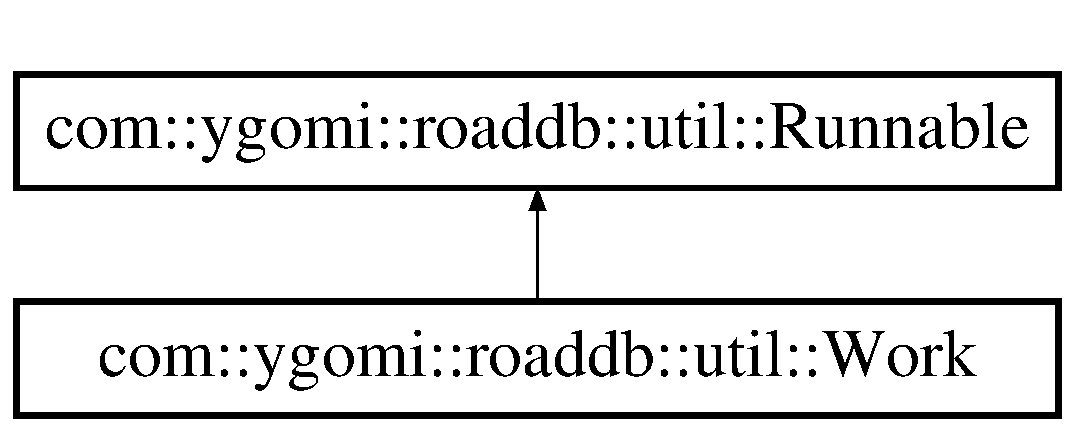
\includegraphics[height=2.000000cm]{classcom_1_1ygomi_1_1roaddb_1_1util_1_1Runnable}
\end{center}
\end{figure}
\subsection*{Public Types}
\begin{DoxyCompactItemize}
\item 
typedef std\-::function$<$ void()$>$ \hyperlink{classcom_1_1ygomi_1_1roaddb_1_1util_1_1Runnable_adc4334b0387442cd2484c3a341ae7fbc}{Func\-Type}
\end{DoxyCompactItemize}
\subsection*{Public Member Functions}
\begin{DoxyCompactItemize}
\item 
\hyperlink{classcom_1_1ygomi_1_1roaddb_1_1util_1_1Runnable_a5f05f2fd37d76573484c68d32f7b5b32}{Runnable} (\hyperlink{classcom_1_1ygomi_1_1roaddb_1_1util_1_1Runnable_adc4334b0387442cd2484c3a341ae7fbc}{Func\-Type} $\ast$func=nullptr)
\item 
virtual \hyperlink{classcom_1_1ygomi_1_1roaddb_1_1util_1_1Runnable_ad64ac814caf458b8cd933a0b8af5e6ae}{$\sim$\-Runnable} ()
\item 
virtual void \hyperlink{classcom_1_1ygomi_1_1roaddb_1_1util_1_1Runnable_a640ed125e4d1f503b6bdec6825fec841}{run} ()
\end{DoxyCompactItemize}


\subsection{Member Typedef Documentation}
\hypertarget{classcom_1_1ygomi_1_1roaddb_1_1util_1_1Runnable_adc4334b0387442cd2484c3a341ae7fbc}{\index{com\-::ygomi\-::roaddb\-::util\-::\-Runnable@{com\-::ygomi\-::roaddb\-::util\-::\-Runnable}!Func\-Type@{Func\-Type}}
\index{Func\-Type@{Func\-Type}!com::ygomi::roaddb::util::Runnable@{com\-::ygomi\-::roaddb\-::util\-::\-Runnable}}
\subsubsection[{Func\-Type}]{\setlength{\rightskip}{0pt plus 5cm}typedef std\-::function$<$void ()$>$ {\bf com\-::ygomi\-::roaddb\-::util\-::\-Runnable\-::\-Func\-Type}}}\label{classcom_1_1ygomi_1_1roaddb_1_1util_1_1Runnable_adc4334b0387442cd2484c3a341ae7fbc}
The signature of the callback function. 

\subsection{Constructor \& Destructor Documentation}
\hypertarget{classcom_1_1ygomi_1_1roaddb_1_1util_1_1Runnable_a5f05f2fd37d76573484c68d32f7b5b32}{\index{com\-::ygomi\-::roaddb\-::util\-::\-Runnable@{com\-::ygomi\-::roaddb\-::util\-::\-Runnable}!Runnable@{Runnable}}
\index{Runnable@{Runnable}!com::ygomi::roaddb::util::Runnable@{com\-::ygomi\-::roaddb\-::util\-::\-Runnable}}
\subsubsection[{Runnable}]{\setlength{\rightskip}{0pt plus 5cm}com\-::ygomi\-::roaddb\-::util\-::\-Runnable\-::\-Runnable (
\begin{DoxyParamCaption}
\item[{{\bf Func\-Type} $\ast$}]{func = {\ttfamily nullptr}}
\end{DoxyParamCaption}
)}}\label{classcom_1_1ygomi_1_1roaddb_1_1util_1_1Runnable_a5f05f2fd37d76573484c68d32f7b5b32}
Constructor


\begin{DoxyParams}{Parameters}
{\em func} & The callback function attached to this work. \\
\hline
\end{DoxyParams}
\hypertarget{classcom_1_1ygomi_1_1roaddb_1_1util_1_1Runnable_ad64ac814caf458b8cd933a0b8af5e6ae}{\index{com\-::ygomi\-::roaddb\-::util\-::\-Runnable@{com\-::ygomi\-::roaddb\-::util\-::\-Runnable}!$\sim$\-Runnable@{$\sim$\-Runnable}}
\index{$\sim$\-Runnable@{$\sim$\-Runnable}!com::ygomi::roaddb::util::Runnable@{com\-::ygomi\-::roaddb\-::util\-::\-Runnable}}
\subsubsection[{$\sim$\-Runnable}]{\setlength{\rightskip}{0pt plus 5cm}com\-::ygomi\-::roaddb\-::util\-::\-Runnable\-::$\sim$\-Runnable (
\begin{DoxyParamCaption}
{}
\end{DoxyParamCaption}
)\hspace{0.3cm}{\ttfamily [virtual]}}}\label{classcom_1_1ygomi_1_1roaddb_1_1util_1_1Runnable_ad64ac814caf458b8cd933a0b8af5e6ae}
Destructor 

\subsection{Member Function Documentation}
\hypertarget{classcom_1_1ygomi_1_1roaddb_1_1util_1_1Runnable_a640ed125e4d1f503b6bdec6825fec841}{\index{com\-::ygomi\-::roaddb\-::util\-::\-Runnable@{com\-::ygomi\-::roaddb\-::util\-::\-Runnable}!run@{run}}
\index{run@{run}!com::ygomi::roaddb::util::Runnable@{com\-::ygomi\-::roaddb\-::util\-::\-Runnable}}
\subsubsection[{run}]{\setlength{\rightskip}{0pt plus 5cm}void com\-::ygomi\-::roaddb\-::util\-::\-Runnable\-::run (
\begin{DoxyParamCaption}
{}
\end{DoxyParamCaption}
)\hspace{0.3cm}{\ttfamily [virtual]}}}\label{classcom_1_1ygomi_1_1roaddb_1_1util_1_1Runnable_a640ed125e4d1f503b6bdec6825fec841}
The method to run this runnable.

Note that once this method is overridden, the function attached will be ineffective, unless it is explicitly invoked in the overridden \hyperlink{classcom_1_1ygomi_1_1roaddb_1_1util_1_1Runnable_a640ed125e4d1f503b6bdec6825fec841}{run()}. 

Reimplemented in \hyperlink{classcom_1_1ygomi_1_1roaddb_1_1util_1_1Work_abc92ca2d3f0b7c7f82ebcb4df0d51d0e}{com\-::ygomi\-::roaddb\-::util\-::\-Work}.



The documentation for this class was generated from the following files\-:\begin{DoxyCompactItemize}
\item 
/opt/db-\/vehicle-\/agent/source/com/ygomi/roaddb/util/Runnable.\-h\item 
/opt/db-\/vehicle-\/agent/source/com/ygomi/roaddb/util/Runnable.\-cpp\end{DoxyCompactItemize}

\hypertarget{classcom_1_1ygomi_1_1roaddb_1_1util_1_1ThreadPool}{\section{com\-:\-:ygomi\-:\-:roaddb\-:\-:util\-:\-:Thread\-Pool Class Reference}
\label{classcom_1_1ygomi_1_1roaddb_1_1util_1_1ThreadPool}\index{com\-::ygomi\-::roaddb\-::util\-::\-Thread\-Pool@{com\-::ygomi\-::roaddb\-::util\-::\-Thread\-Pool}}
}
\subsection*{Public Member Functions}
\begin{DoxyCompactItemize}
\item 
\hyperlink{classcom_1_1ygomi_1_1roaddb_1_1util_1_1ThreadPool_ac08fb558f6e484ebbf680d94104009d4}{Thread\-Pool} (uint32\-\_\-t size=8)
\item 
virtual \hyperlink{classcom_1_1ygomi_1_1roaddb_1_1util_1_1ThreadPool_a8d99bb4e9986d3c817d0c8781da80e22}{$\sim$\-Thread\-Pool} ()
\item 
virtual uint32\-\_\-t \hyperlink{classcom_1_1ygomi_1_1roaddb_1_1util_1_1ThreadPool_a70ba5922908b606d2a0b24da904566fb}{get\-Size} ()
\item 
virtual uint32\-\_\-t \hyperlink{classcom_1_1ygomi_1_1roaddb_1_1util_1_1ThreadPool_aa3955a1e2512c96535f137a6bc72aec0}{get\-Idle\-Count} ()
\item 
virtual \hyperlink{classcom_1_1ygomi_1_1roaddb_1_1util_1_1WorkThread}{Work\-Thread} $\ast$ \hyperlink{classcom_1_1ygomi_1_1roaddb_1_1util_1_1ThreadPool_a042c27046d92f2e389e77fe52d4dc0d2}{fetch} ()
\end{DoxyCompactItemize}
\subsection*{Friends}
\begin{DoxyCompactItemize}
\item 
\hypertarget{classcom_1_1ygomi_1_1roaddb_1_1util_1_1ThreadPool_a47faa4de4512428060e1fe5c768b4d47}{class {\bfseries Work\-Thread}}\label{classcom_1_1ygomi_1_1roaddb_1_1util_1_1ThreadPool_a47faa4de4512428060e1fe5c768b4d47}

\end{DoxyCompactItemize}


\subsection{Constructor \& Destructor Documentation}
\hypertarget{classcom_1_1ygomi_1_1roaddb_1_1util_1_1ThreadPool_ac08fb558f6e484ebbf680d94104009d4}{\index{com\-::ygomi\-::roaddb\-::util\-::\-Thread\-Pool@{com\-::ygomi\-::roaddb\-::util\-::\-Thread\-Pool}!Thread\-Pool@{Thread\-Pool}}
\index{Thread\-Pool@{Thread\-Pool}!com::ygomi::roaddb::util::ThreadPool@{com\-::ygomi\-::roaddb\-::util\-::\-Thread\-Pool}}
\subsubsection[{Thread\-Pool}]{\setlength{\rightskip}{0pt plus 5cm}com\-::ygomi\-::roaddb\-::util\-::\-Thread\-Pool\-::\-Thread\-Pool (
\begin{DoxyParamCaption}
\item[{uint32\-\_\-t}]{size = {\ttfamily 8}}
\end{DoxyParamCaption}
)\hspace{0.3cm}{\ttfamily [explicit]}}}\label{classcom_1_1ygomi_1_1roaddb_1_1util_1_1ThreadPool_ac08fb558f6e484ebbf680d94104009d4}
Constructor


\begin{DoxyParams}{Parameters}
{\em max\-Size} & The size of the thread pool. Default value is 8. \\
\hline
\end{DoxyParams}
\hypertarget{classcom_1_1ygomi_1_1roaddb_1_1util_1_1ThreadPool_a8d99bb4e9986d3c817d0c8781da80e22}{\index{com\-::ygomi\-::roaddb\-::util\-::\-Thread\-Pool@{com\-::ygomi\-::roaddb\-::util\-::\-Thread\-Pool}!$\sim$\-Thread\-Pool@{$\sim$\-Thread\-Pool}}
\index{$\sim$\-Thread\-Pool@{$\sim$\-Thread\-Pool}!com::ygomi::roaddb::util::ThreadPool@{com\-::ygomi\-::roaddb\-::util\-::\-Thread\-Pool}}
\subsubsection[{$\sim$\-Thread\-Pool}]{\setlength{\rightskip}{0pt plus 5cm}com\-::ygomi\-::roaddb\-::util\-::\-Thread\-Pool\-::$\sim$\-Thread\-Pool (
\begin{DoxyParamCaption}
{}
\end{DoxyParamCaption}
)\hspace{0.3cm}{\ttfamily [virtual]}}}\label{classcom_1_1ygomi_1_1roaddb_1_1util_1_1ThreadPool_a8d99bb4e9986d3c817d0c8781da80e22}
Destructor 

\subsection{Member Function Documentation}
\hypertarget{classcom_1_1ygomi_1_1roaddb_1_1util_1_1ThreadPool_a042c27046d92f2e389e77fe52d4dc0d2}{\index{com\-::ygomi\-::roaddb\-::util\-::\-Thread\-Pool@{com\-::ygomi\-::roaddb\-::util\-::\-Thread\-Pool}!fetch@{fetch}}
\index{fetch@{fetch}!com::ygomi::roaddb::util::ThreadPool@{com\-::ygomi\-::roaddb\-::util\-::\-Thread\-Pool}}
\subsubsection[{fetch}]{\setlength{\rightskip}{0pt plus 5cm}{\bf Work\-Thread} $\ast$ com\-::ygomi\-::roaddb\-::util\-::\-Thread\-Pool\-::fetch (
\begin{DoxyParamCaption}
{}
\end{DoxyParamCaption}
)\hspace{0.3cm}{\ttfamily [virtual]}}}\label{classcom_1_1ygomi_1_1roaddb_1_1util_1_1ThreadPool_a042c27046d92f2e389e77fe52d4dc0d2}
Fetch an idle thread from the thread pool.

\begin{DoxyReturn}{Returns}
The pointer to the idle thread, or null if no idle thread available. 
\end{DoxyReturn}
\hypertarget{classcom_1_1ygomi_1_1roaddb_1_1util_1_1ThreadPool_aa3955a1e2512c96535f137a6bc72aec0}{\index{com\-::ygomi\-::roaddb\-::util\-::\-Thread\-Pool@{com\-::ygomi\-::roaddb\-::util\-::\-Thread\-Pool}!get\-Idle\-Count@{get\-Idle\-Count}}
\index{get\-Idle\-Count@{get\-Idle\-Count}!com::ygomi::roaddb::util::ThreadPool@{com\-::ygomi\-::roaddb\-::util\-::\-Thread\-Pool}}
\subsubsection[{get\-Idle\-Count}]{\setlength{\rightskip}{0pt plus 5cm}virtual uint32\-\_\-t com\-::ygomi\-::roaddb\-::util\-::\-Thread\-Pool\-::get\-Idle\-Count (
\begin{DoxyParamCaption}
{}
\end{DoxyParamCaption}
)\hspace{0.3cm}{\ttfamily [inline]}, {\ttfamily [virtual]}}}\label{classcom_1_1ygomi_1_1roaddb_1_1util_1_1ThreadPool_aa3955a1e2512c96535f137a6bc72aec0}
The count of idle threads.

\begin{DoxyReturn}{Returns}
The count of idle threads. 
\end{DoxyReturn}
\hypertarget{classcom_1_1ygomi_1_1roaddb_1_1util_1_1ThreadPool_a70ba5922908b606d2a0b24da904566fb}{\index{com\-::ygomi\-::roaddb\-::util\-::\-Thread\-Pool@{com\-::ygomi\-::roaddb\-::util\-::\-Thread\-Pool}!get\-Size@{get\-Size}}
\index{get\-Size@{get\-Size}!com::ygomi::roaddb::util::ThreadPool@{com\-::ygomi\-::roaddb\-::util\-::\-Thread\-Pool}}
\subsubsection[{get\-Size}]{\setlength{\rightskip}{0pt plus 5cm}virtual uint32\-\_\-t com\-::ygomi\-::roaddb\-::util\-::\-Thread\-Pool\-::get\-Size (
\begin{DoxyParamCaption}
{}
\end{DoxyParamCaption}
)\hspace{0.3cm}{\ttfamily [inline]}, {\ttfamily [virtual]}}}\label{classcom_1_1ygomi_1_1roaddb_1_1util_1_1ThreadPool_a70ba5922908b606d2a0b24da904566fb}
The size of the thread pool.

\begin{DoxyReturn}{Returns}
The size of the thread pool. 
\end{DoxyReturn}


The documentation for this class was generated from the following files\-:\begin{DoxyCompactItemize}
\item 
/opt/db-\/vehicle-\/agent/source/com/ygomi/roaddb/util/Thread\-Pool.\-h\item 
/opt/db-\/vehicle-\/agent/source/com/ygomi/roaddb/util/Thread\-Pool.\-cpp\end{DoxyCompactItemize}

\hypertarget{classcom_1_1ygomi_1_1roaddb_1_1util_1_1TSQueue}{\section{com\-:\-:ygomi\-:\-:roaddb\-:\-:util\-:\-:T\-S\-Queue$<$ T $>$ Class Template Reference}
\label{classcom_1_1ygomi_1_1roaddb_1_1util_1_1TSQueue}\index{com\-::ygomi\-::roaddb\-::util\-::\-T\-S\-Queue$<$ T $>$@{com\-::ygomi\-::roaddb\-::util\-::\-T\-S\-Queue$<$ T $>$}}
}
\subsection*{Public Types}
\begin{DoxyCompactItemize}
\item 
typedef std\-::function$<$ void(\hyperlink{classcom_1_1ygomi_1_1roaddb_1_1util_1_1TSQueue}{T\-S\-Queue}\\*
$<$ T $>$ $\ast$)$>$ \hyperlink{classcom_1_1ygomi_1_1roaddb_1_1util_1_1TSQueue_aa81eeb34e0d4b311c71838a14fce7e2f}{Callback\-Type}
\end{DoxyCompactItemize}
\subsection*{Public Member Functions}
\begin{DoxyCompactItemize}
\item 
\hyperlink{classcom_1_1ygomi_1_1roaddb_1_1util_1_1TSQueue_a8671f03fd0e0cb6343b4320eceaad756}{T\-S\-Queue} (uint32\-\_\-t max\-Size=32)
\item 
virtual \hyperlink{classcom_1_1ygomi_1_1roaddb_1_1util_1_1TSQueue_ae6cd63f91b3f8acfc2fb024a0f502b78}{$\sim$\-T\-S\-Queue} ()
\item 
bool \hyperlink{classcom_1_1ygomi_1_1roaddb_1_1util_1_1TSQueue_abcc079279d8a9ea9e893688a8091f2d1}{empty} () const 
\item 
int \hyperlink{classcom_1_1ygomi_1_1roaddb_1_1util_1_1TSQueue_a93b080b3e5d2826b8935bc99c84cbc85}{get\-Max\-Size} () const 
\item 
int \hyperlink{classcom_1_1ygomi_1_1roaddb_1_1util_1_1TSQueue_a793306954e163e23bcfe097f85667821}{size} () const 
\item 
bool \hyperlink{classcom_1_1ygomi_1_1roaddb_1_1util_1_1TSQueue_af9932c6261a05455ddba853cb7f07ddd}{enqueue} (std\-::shared\-\_\-ptr$<$ T $>$ element)
\item 
std\-::shared\-\_\-ptr$<$ T $>$ \hyperlink{classcom_1_1ygomi_1_1roaddb_1_1util_1_1TSQueue_ab04c41abb275f83c8fb1ac0b723a8de5}{dequeue} ()
\item 
void \hyperlink{classcom_1_1ygomi_1_1roaddb_1_1util_1_1TSQueue_a505f5fee729f59577303267f0dfe5f40}{add\-Enqueue\-Listener} (\hyperlink{classcom_1_1ygomi_1_1roaddb_1_1util_1_1TSQueue_aa81eeb34e0d4b311c71838a14fce7e2f}{Callback\-Type} $\ast$callback)
\item 
void \hyperlink{classcom_1_1ygomi_1_1roaddb_1_1util_1_1TSQueue_a4cb1849202ceda7adcb0a3aab004a3cf}{clear\-Enqueue\-Listener} ()
\end{DoxyCompactItemize}


\subsection{Member Typedef Documentation}
\hypertarget{classcom_1_1ygomi_1_1roaddb_1_1util_1_1TSQueue_aa81eeb34e0d4b311c71838a14fce7e2f}{\index{com\-::ygomi\-::roaddb\-::util\-::\-T\-S\-Queue@{com\-::ygomi\-::roaddb\-::util\-::\-T\-S\-Queue}!Callback\-Type@{Callback\-Type}}
\index{Callback\-Type@{Callback\-Type}!com::ygomi::roaddb::util::TSQueue@{com\-::ygomi\-::roaddb\-::util\-::\-T\-S\-Queue}}
\subsubsection[{Callback\-Type}]{\setlength{\rightskip}{0pt plus 5cm}template$<$class T$>$ typedef std\-::function$<$void ({\bf T\-S\-Queue}$<$T$>$$\ast$)$>$ {\bf com\-::ygomi\-::roaddb\-::util\-::\-T\-S\-Queue}$<$ T $>$\-::{\bf Callback\-Type}}}\label{classcom_1_1ygomi_1_1roaddb_1_1util_1_1TSQueue_aa81eeb34e0d4b311c71838a14fce7e2f}
Type definition for callback function invoked when a new element is enqueued. 

\subsection{Constructor \& Destructor Documentation}
\hypertarget{classcom_1_1ygomi_1_1roaddb_1_1util_1_1TSQueue_a8671f03fd0e0cb6343b4320eceaad756}{\index{com\-::ygomi\-::roaddb\-::util\-::\-T\-S\-Queue@{com\-::ygomi\-::roaddb\-::util\-::\-T\-S\-Queue}!T\-S\-Queue@{T\-S\-Queue}}
\index{T\-S\-Queue@{T\-S\-Queue}!com::ygomi::roaddb::util::TSQueue@{com\-::ygomi\-::roaddb\-::util\-::\-T\-S\-Queue}}
\subsubsection[{T\-S\-Queue}]{\setlength{\rightskip}{0pt plus 5cm}template$<$class T$>$ {\bf com\-::ygomi\-::roaddb\-::util\-::\-T\-S\-Queue}$<$ T $>$\-::{\bf T\-S\-Queue} (
\begin{DoxyParamCaption}
\item[{uint32\-\_\-t}]{max\-Size = {\ttfamily 32}}
\end{DoxyParamCaption}
)\hspace{0.3cm}{\ttfamily [inline]}}}\label{classcom_1_1ygomi_1_1roaddb_1_1util_1_1TSQueue_a8671f03fd0e0cb6343b4320eceaad756}
Constructor


\begin{DoxyParams}{Parameters}
{\em max\-Size} & The max size of the queue. \\
\hline
\end{DoxyParams}
\hypertarget{classcom_1_1ygomi_1_1roaddb_1_1util_1_1TSQueue_ae6cd63f91b3f8acfc2fb024a0f502b78}{\index{com\-::ygomi\-::roaddb\-::util\-::\-T\-S\-Queue@{com\-::ygomi\-::roaddb\-::util\-::\-T\-S\-Queue}!$\sim$\-T\-S\-Queue@{$\sim$\-T\-S\-Queue}}
\index{$\sim$\-T\-S\-Queue@{$\sim$\-T\-S\-Queue}!com::ygomi::roaddb::util::TSQueue@{com\-::ygomi\-::roaddb\-::util\-::\-T\-S\-Queue}}
\subsubsection[{$\sim$\-T\-S\-Queue}]{\setlength{\rightskip}{0pt plus 5cm}template$<$class T$>$ virtual {\bf com\-::ygomi\-::roaddb\-::util\-::\-T\-S\-Queue}$<$ T $>$\-::$\sim${\bf T\-S\-Queue} (
\begin{DoxyParamCaption}
{}
\end{DoxyParamCaption}
)\hspace{0.3cm}{\ttfamily [inline]}, {\ttfamily [virtual]}}}\label{classcom_1_1ygomi_1_1roaddb_1_1util_1_1TSQueue_ae6cd63f91b3f8acfc2fb024a0f502b78}
Destructor 

\subsection{Member Function Documentation}
\hypertarget{classcom_1_1ygomi_1_1roaddb_1_1util_1_1TSQueue_a505f5fee729f59577303267f0dfe5f40}{\index{com\-::ygomi\-::roaddb\-::util\-::\-T\-S\-Queue@{com\-::ygomi\-::roaddb\-::util\-::\-T\-S\-Queue}!add\-Enqueue\-Listener@{add\-Enqueue\-Listener}}
\index{add\-Enqueue\-Listener@{add\-Enqueue\-Listener}!com::ygomi::roaddb::util::TSQueue@{com\-::ygomi\-::roaddb\-::util\-::\-T\-S\-Queue}}
\subsubsection[{add\-Enqueue\-Listener}]{\setlength{\rightskip}{0pt plus 5cm}template$<$class T$>$ void {\bf com\-::ygomi\-::roaddb\-::util\-::\-T\-S\-Queue}$<$ T $>$\-::add\-Enqueue\-Listener (
\begin{DoxyParamCaption}
\item[{{\bf Callback\-Type} $\ast$}]{callback}
\end{DoxyParamCaption}
)\hspace{0.3cm}{\ttfamily [inline]}}}\label{classcom_1_1ygomi_1_1roaddb_1_1util_1_1TSQueue_a505f5fee729f59577303267f0dfe5f40}
Register enqueue listener callback function which will be invoked at \hyperlink{classcom_1_1ygomi_1_1roaddb_1_1util_1_1TSQueue_af9932c6261a05455ddba853cb7f07ddd}{enqueue()}.


\begin{DoxyParams}{Parameters}
{\em callback} & The callback function.\\
\hline
\end{DoxyParams}
Note the callback function is normally used to notify the thread which is waiting on the queue. \hypertarget{classcom_1_1ygomi_1_1roaddb_1_1util_1_1TSQueue_a4cb1849202ceda7adcb0a3aab004a3cf}{\index{com\-::ygomi\-::roaddb\-::util\-::\-T\-S\-Queue@{com\-::ygomi\-::roaddb\-::util\-::\-T\-S\-Queue}!clear\-Enqueue\-Listener@{clear\-Enqueue\-Listener}}
\index{clear\-Enqueue\-Listener@{clear\-Enqueue\-Listener}!com::ygomi::roaddb::util::TSQueue@{com\-::ygomi\-::roaddb\-::util\-::\-T\-S\-Queue}}
\subsubsection[{clear\-Enqueue\-Listener}]{\setlength{\rightskip}{0pt plus 5cm}template$<$class T$>$ void {\bf com\-::ygomi\-::roaddb\-::util\-::\-T\-S\-Queue}$<$ T $>$\-::clear\-Enqueue\-Listener (
\begin{DoxyParamCaption}
{}
\end{DoxyParamCaption}
)\hspace{0.3cm}{\ttfamily [inline]}}}\label{classcom_1_1ygomi_1_1roaddb_1_1util_1_1TSQueue_a4cb1849202ceda7adcb0a3aab004a3cf}
Clear all enqueue listener callback functions. \hypertarget{classcom_1_1ygomi_1_1roaddb_1_1util_1_1TSQueue_ab04c41abb275f83c8fb1ac0b723a8de5}{\index{com\-::ygomi\-::roaddb\-::util\-::\-T\-S\-Queue@{com\-::ygomi\-::roaddb\-::util\-::\-T\-S\-Queue}!dequeue@{dequeue}}
\index{dequeue@{dequeue}!com::ygomi::roaddb::util::TSQueue@{com\-::ygomi\-::roaddb\-::util\-::\-T\-S\-Queue}}
\subsubsection[{dequeue}]{\setlength{\rightskip}{0pt plus 5cm}template$<$class T$>$ std\-::shared\-\_\-ptr$<$T$>$ {\bf com\-::ygomi\-::roaddb\-::util\-::\-T\-S\-Queue}$<$ T $>$\-::dequeue (
\begin{DoxyParamCaption}
{}
\end{DoxyParamCaption}
)\hspace{0.3cm}{\ttfamily [inline]}}}\label{classcom_1_1ygomi_1_1roaddb_1_1util_1_1TSQueue_ab04c41abb275f83c8fb1ac0b723a8de5}
Pop the first element of the queue.

\begin{DoxyReturn}{Returns}
Return the first element of the queue if the queue is not empty, or return null. 
\end{DoxyReturn}
\hypertarget{classcom_1_1ygomi_1_1roaddb_1_1util_1_1TSQueue_abcc079279d8a9ea9e893688a8091f2d1}{\index{com\-::ygomi\-::roaddb\-::util\-::\-T\-S\-Queue@{com\-::ygomi\-::roaddb\-::util\-::\-T\-S\-Queue}!empty@{empty}}
\index{empty@{empty}!com::ygomi::roaddb::util::TSQueue@{com\-::ygomi\-::roaddb\-::util\-::\-T\-S\-Queue}}
\subsubsection[{empty}]{\setlength{\rightskip}{0pt plus 5cm}template$<$class T$>$ bool {\bf com\-::ygomi\-::roaddb\-::util\-::\-T\-S\-Queue}$<$ T $>$\-::empty (
\begin{DoxyParamCaption}
{}
\end{DoxyParamCaption}
) const\hspace{0.3cm}{\ttfamily [inline]}}}\label{classcom_1_1ygomi_1_1roaddb_1_1util_1_1TSQueue_abcc079279d8a9ea9e893688a8091f2d1}
If the queue is empty.

\begin{DoxyReturn}{Returns}
True if empty, false otherwise. 
\end{DoxyReturn}
\hypertarget{classcom_1_1ygomi_1_1roaddb_1_1util_1_1TSQueue_af9932c6261a05455ddba853cb7f07ddd}{\index{com\-::ygomi\-::roaddb\-::util\-::\-T\-S\-Queue@{com\-::ygomi\-::roaddb\-::util\-::\-T\-S\-Queue}!enqueue@{enqueue}}
\index{enqueue@{enqueue}!com::ygomi::roaddb::util::TSQueue@{com\-::ygomi\-::roaddb\-::util\-::\-T\-S\-Queue}}
\subsubsection[{enqueue}]{\setlength{\rightskip}{0pt plus 5cm}template$<$class T$>$ bool {\bf com\-::ygomi\-::roaddb\-::util\-::\-T\-S\-Queue}$<$ T $>$\-::enqueue (
\begin{DoxyParamCaption}
\item[{std\-::shared\-\_\-ptr$<$ T $>$}]{element}
\end{DoxyParamCaption}
)\hspace{0.3cm}{\ttfamily [inline]}}}\label{classcom_1_1ygomi_1_1roaddb_1_1util_1_1TSQueue_af9932c6261a05455ddba853cb7f07ddd}
Push a new element into the queue.


\begin{DoxyParams}{Parameters}
{\em element} & The element to be pushed. Note the element must be a pointer.\\
\hline
\end{DoxyParams}
Note The callback function will be invoked here if it is registered. \hypertarget{classcom_1_1ygomi_1_1roaddb_1_1util_1_1TSQueue_a93b080b3e5d2826b8935bc99c84cbc85}{\index{com\-::ygomi\-::roaddb\-::util\-::\-T\-S\-Queue@{com\-::ygomi\-::roaddb\-::util\-::\-T\-S\-Queue}!get\-Max\-Size@{get\-Max\-Size}}
\index{get\-Max\-Size@{get\-Max\-Size}!com::ygomi::roaddb::util::TSQueue@{com\-::ygomi\-::roaddb\-::util\-::\-T\-S\-Queue}}
\subsubsection[{get\-Max\-Size}]{\setlength{\rightskip}{0pt plus 5cm}template$<$class T$>$ int {\bf com\-::ygomi\-::roaddb\-::util\-::\-T\-S\-Queue}$<$ T $>$\-::get\-Max\-Size (
\begin{DoxyParamCaption}
{}
\end{DoxyParamCaption}
) const\hspace{0.3cm}{\ttfamily [inline]}}}\label{classcom_1_1ygomi_1_1roaddb_1_1util_1_1TSQueue_a93b080b3e5d2826b8935bc99c84cbc85}
Get the maximum size of the queue.

\begin{DoxyReturn}{Returns}
The maximum size of the queue. 
\end{DoxyReturn}
\hypertarget{classcom_1_1ygomi_1_1roaddb_1_1util_1_1TSQueue_a793306954e163e23bcfe097f85667821}{\index{com\-::ygomi\-::roaddb\-::util\-::\-T\-S\-Queue@{com\-::ygomi\-::roaddb\-::util\-::\-T\-S\-Queue}!size@{size}}
\index{size@{size}!com::ygomi::roaddb::util::TSQueue@{com\-::ygomi\-::roaddb\-::util\-::\-T\-S\-Queue}}
\subsubsection[{size}]{\setlength{\rightskip}{0pt plus 5cm}template$<$class T$>$ int {\bf com\-::ygomi\-::roaddb\-::util\-::\-T\-S\-Queue}$<$ T $>$\-::size (
\begin{DoxyParamCaption}
{}
\end{DoxyParamCaption}
) const\hspace{0.3cm}{\ttfamily [inline]}}}\label{classcom_1_1ygomi_1_1roaddb_1_1util_1_1TSQueue_a793306954e163e23bcfe097f85667821}
Get the size of the queue.

\begin{DoxyReturn}{Returns}
The size (number of elements) of the queue. 
\end{DoxyReturn}


The documentation for this class was generated from the following file\-:\begin{DoxyCompactItemize}
\item 
/opt/db-\/vehicle-\/agent/source/com/ygomi/roaddb/util/T\-S\-Queue.\-hpp\end{DoxyCompactItemize}

\hypertarget{classcom_1_1ygomi_1_1roaddb_1_1util_1_1Work}{\section{com\-:\-:ygomi\-:\-:roaddb\-:\-:util\-:\-:Work Class Reference}
\label{classcom_1_1ygomi_1_1roaddb_1_1util_1_1Work}\index{com\-::ygomi\-::roaddb\-::util\-::\-Work@{com\-::ygomi\-::roaddb\-::util\-::\-Work}}
}
Inheritance diagram for com\-:\-:ygomi\-:\-:roaddb\-:\-:util\-:\-:Work\-:\begin{figure}[H]
\begin{center}
\leavevmode
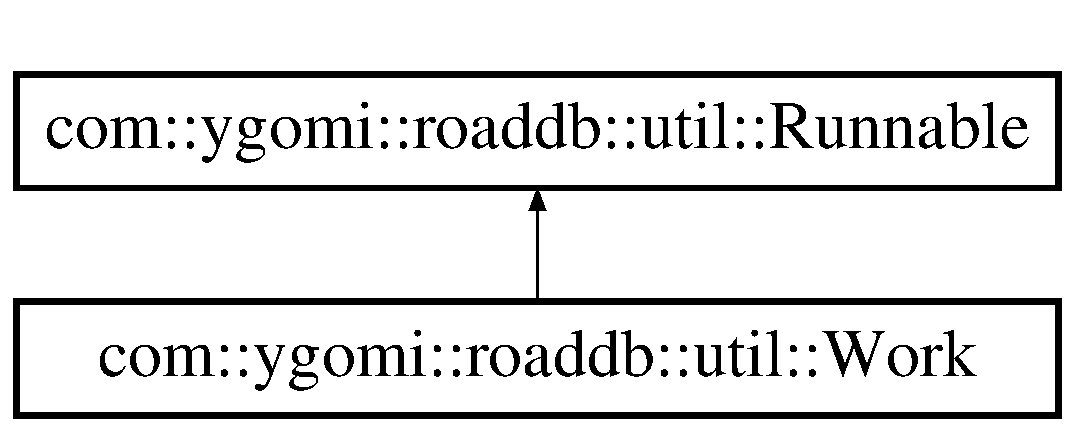
\includegraphics[height=2.000000cm]{classcom_1_1ygomi_1_1roaddb_1_1util_1_1Work}
\end{center}
\end{figure}
\subsection*{Public Member Functions}
\begin{DoxyCompactItemize}
\item 
\hypertarget{classcom_1_1ygomi_1_1roaddb_1_1util_1_1Work_acee5d8a147fc89e9adf6c640580a3580}{{\bfseries Work} (\hyperlink{classcom_1_1ygomi_1_1roaddb_1_1util_1_1Runnable_adc4334b0387442cd2484c3a341ae7fbc}{Func\-Type} $\ast$func=nullptr)}\label{classcom_1_1ygomi_1_1roaddb_1_1util_1_1Work_acee5d8a147fc89e9adf6c640580a3580}

\item 
virtual void \hyperlink{classcom_1_1ygomi_1_1roaddb_1_1util_1_1Work_abc92ca2d3f0b7c7f82ebcb4df0d51d0e}{run} ()
\item 
\hypertarget{classcom_1_1ygomi_1_1roaddb_1_1util_1_1Work_af33ed777921f156941b150a64e4f6d94}{std\-::shared\-\_\-ptr$<$ \hyperlink{classcom_1_1ygomi_1_1roaddb_1_1util_1_1Message}{Message} $>$ {\bfseries get\-Input\-Msg} ()}\label{classcom_1_1ygomi_1_1roaddb_1_1util_1_1Work_af33ed777921f156941b150a64e4f6d94}

\item 
\hypertarget{classcom_1_1ygomi_1_1roaddb_1_1util_1_1Work_a6b8aff938d51ca3619efc1f92b6725d0}{std\-::shared\-\_\-ptr$<$ \hyperlink{classcom_1_1ygomi_1_1roaddb_1_1util_1_1Message}{Message} $>$ {\bfseries get\-Output\-Msg} ()}\label{classcom_1_1ygomi_1_1roaddb_1_1util_1_1Work_a6b8aff938d51ca3619efc1f92b6725d0}

\item 
\hypertarget{classcom_1_1ygomi_1_1roaddb_1_1util_1_1Work_a5b0bf836c6a4048bdb24f6f55b7b10bc}{void {\bfseries set\-Input\-Msg} (std\-::shared\-\_\-ptr$<$ \hyperlink{classcom_1_1ygomi_1_1roaddb_1_1util_1_1Message}{Message} $>$ input\-Msg)}\label{classcom_1_1ygomi_1_1roaddb_1_1util_1_1Work_a5b0bf836c6a4048bdb24f6f55b7b10bc}

\item 
\hypertarget{classcom_1_1ygomi_1_1roaddb_1_1util_1_1Work_aaf99d410083eab55ce6872ece28c1678}{void {\bfseries set\-Output\-Msg} (std\-::shared\-\_\-ptr$<$ \hyperlink{classcom_1_1ygomi_1_1roaddb_1_1util_1_1Message}{Message} $>$ output\-Msg)}\label{classcom_1_1ygomi_1_1roaddb_1_1util_1_1Work_aaf99d410083eab55ce6872ece28c1678}

\end{DoxyCompactItemize}
\subsection*{Additional Inherited Members}


\subsection{Member Function Documentation}
\hypertarget{classcom_1_1ygomi_1_1roaddb_1_1util_1_1Work_abc92ca2d3f0b7c7f82ebcb4df0d51d0e}{\index{com\-::ygomi\-::roaddb\-::util\-::\-Work@{com\-::ygomi\-::roaddb\-::util\-::\-Work}!run@{run}}
\index{run@{run}!com::ygomi::roaddb::util::Work@{com\-::ygomi\-::roaddb\-::util\-::\-Work}}
\subsubsection[{run}]{\setlength{\rightskip}{0pt plus 5cm}void com\-::ygomi\-::roaddb\-::util\-::\-Work\-::run (
\begin{DoxyParamCaption}
{}
\end{DoxyParamCaption}
)\hspace{0.3cm}{\ttfamily [virtual]}}}\label{classcom_1_1ygomi_1_1roaddb_1_1util_1_1Work_abc92ca2d3f0b7c7f82ebcb4df0d51d0e}
The method to run this runnable.

Note that once this method is overridden, the function attached will be ineffective, unless it is explicitly invoked in the overridden \hyperlink{classcom_1_1ygomi_1_1roaddb_1_1util_1_1Work_abc92ca2d3f0b7c7f82ebcb4df0d51d0e}{run()}. 

Reimplemented from \hyperlink{classcom_1_1ygomi_1_1roaddb_1_1util_1_1Runnable_a640ed125e4d1f503b6bdec6825fec841}{com\-::ygomi\-::roaddb\-::util\-::\-Runnable}.



The documentation for this class was generated from the following files\-:\begin{DoxyCompactItemize}
\item 
/opt/db-\/vehicle-\/agent/source/com/ygomi/roaddb/util/Work.\-h\item 
/opt/db-\/vehicle-\/agent/source/com/ygomi/roaddb/util/Work.\-cpp\end{DoxyCompactItemize}

\hypertarget{classcom_1_1ygomi_1_1roaddb_1_1util_1_1WorkThread}{\section{com\-:\-:ygomi\-:\-:roaddb\-:\-:util\-:\-:Work\-Thread Class Reference}
\label{classcom_1_1ygomi_1_1roaddb_1_1util_1_1WorkThread}\index{com\-::ygomi\-::roaddb\-::util\-::\-Work\-Thread@{com\-::ygomi\-::roaddb\-::util\-::\-Work\-Thread}}
}
\subsection*{Public Member Functions}
\begin{DoxyCompactItemize}
\item 
virtual \hyperlink{classcom_1_1ygomi_1_1roaddb_1_1util_1_1WorkThread_a0ec3db7dda670d07dd3ed080f2d7e40c}{$\sim$\-Work\-Thread} ()
\item 
virtual int \hyperlink{classcom_1_1ygomi_1_1roaddb_1_1util_1_1WorkThread_a4ecf08df35765b316742bf32f24b6cf0}{get\-Status} () const 
\item 
virtual void \hyperlink{classcom_1_1ygomi_1_1roaddb_1_1util_1_1WorkThread_afadf70a2f873ad2a5119c98467e8cc19}{do\-Work} (std\-::shared\-\_\-ptr$<$ \hyperlink{classcom_1_1ygomi_1_1roaddb_1_1util_1_1Work}{Work} $>$ work)
\end{DoxyCompactItemize}
\subsection*{Static Public Attributes}
\begin{DoxyCompactItemize}
\item 
static const int \hyperlink{classcom_1_1ygomi_1_1roaddb_1_1util_1_1WorkThread_a327f2a2fcfd8a63f1684e6a7f4139558}{S\-T\-A\-T\-U\-S\-\_\-\-I\-N\-I\-T} = 1
\item 
static const int \hyperlink{classcom_1_1ygomi_1_1roaddb_1_1util_1_1WorkThread_ad6bc7481694d9df02ebcd1b827abb755}{S\-T\-A\-T\-U\-S\-\_\-\-I\-D\-L\-E} = 2
\item 
static const int \hyperlink{classcom_1_1ygomi_1_1roaddb_1_1util_1_1WorkThread_a7db27d123b3e2f4c5512bad8cbb67aee}{S\-T\-A\-T\-U\-S\-\_\-\-W\-O\-R\-K\-I\-N\-G} = 3
\item 
static const int \hyperlink{classcom_1_1ygomi_1_1roaddb_1_1util_1_1WorkThread_a936330c526d2a547c63831d9596acb53}{S\-T\-A\-T\-U\-S\-\_\-\-T\-E\-R\-M\-I\-N\-A\-T\-E\-D} = 4
\end{DoxyCompactItemize}
\subsection*{Friends}
\begin{DoxyCompactItemize}
\item 
\hypertarget{classcom_1_1ygomi_1_1roaddb_1_1util_1_1WorkThread_a5d97748be7d69dcc44ef551ea35ef20f}{class {\bfseries Thread\-Pool}}\label{classcom_1_1ygomi_1_1roaddb_1_1util_1_1WorkThread_a5d97748be7d69dcc44ef551ea35ef20f}

\end{DoxyCompactItemize}


\subsection{Constructor \& Destructor Documentation}
\hypertarget{classcom_1_1ygomi_1_1roaddb_1_1util_1_1WorkThread_a0ec3db7dda670d07dd3ed080f2d7e40c}{\index{com\-::ygomi\-::roaddb\-::util\-::\-Work\-Thread@{com\-::ygomi\-::roaddb\-::util\-::\-Work\-Thread}!$\sim$\-Work\-Thread@{$\sim$\-Work\-Thread}}
\index{$\sim$\-Work\-Thread@{$\sim$\-Work\-Thread}!com::ygomi::roaddb::util::WorkThread@{com\-::ygomi\-::roaddb\-::util\-::\-Work\-Thread}}
\subsubsection[{$\sim$\-Work\-Thread}]{\setlength{\rightskip}{0pt plus 5cm}com\-::ygomi\-::roaddb\-::util\-::\-Work\-Thread\-::$\sim$\-Work\-Thread (
\begin{DoxyParamCaption}
{}
\end{DoxyParamCaption}
)\hspace{0.3cm}{\ttfamily [virtual]}}}\label{classcom_1_1ygomi_1_1roaddb_1_1util_1_1WorkThread_a0ec3db7dda670d07dd3ed080f2d7e40c}
Destructor 

\subsection{Member Function Documentation}
\hypertarget{classcom_1_1ygomi_1_1roaddb_1_1util_1_1WorkThread_afadf70a2f873ad2a5119c98467e8cc19}{\index{com\-::ygomi\-::roaddb\-::util\-::\-Work\-Thread@{com\-::ygomi\-::roaddb\-::util\-::\-Work\-Thread}!do\-Work@{do\-Work}}
\index{do\-Work@{do\-Work}!com::ygomi::roaddb::util::WorkThread@{com\-::ygomi\-::roaddb\-::util\-::\-Work\-Thread}}
\subsubsection[{do\-Work}]{\setlength{\rightskip}{0pt plus 5cm}void com\-::ygomi\-::roaddb\-::util\-::\-Work\-Thread\-::do\-Work (
\begin{DoxyParamCaption}
\item[{std\-::shared\-\_\-ptr$<$ {\bf Work} $>$}]{work}
\end{DoxyParamCaption}
)\hspace{0.3cm}{\ttfamily [virtual]}}}\label{classcom_1_1ygomi_1_1roaddb_1_1util_1_1WorkThread_afadf70a2f873ad2a5119c98467e8cc19}
Start to do some work.


\begin{DoxyParams}{Parameters}
{\em I\-N\mbox{]}} & work The work to do.\\
\hline
\end{DoxyParams}
Notes\-:
\begin{DoxyEnumerate}
\item This method will resume this work thread (while it is suspended) and let it do the given work.
\item This method only takes effect when the status of this work thread is S\-T\-A\-T\-U\-S\-\_\-\-I\-D\-L\-E, or nothing will happen.
\item After this work thread is resumed by this method, the status will become S\-T\-A\-T\-U\-S\-\_\-\-W\-O\-R\-K\-I\-N\-G; and once the work is done, the status will change back to S\-T\-A\-T\-U\-S\-\_\-\-I\-D\-L\-E and this work thread will be suspended again. 
\end{DoxyEnumerate}\hypertarget{classcom_1_1ygomi_1_1roaddb_1_1util_1_1WorkThread_a4ecf08df35765b316742bf32f24b6cf0}{\index{com\-::ygomi\-::roaddb\-::util\-::\-Work\-Thread@{com\-::ygomi\-::roaddb\-::util\-::\-Work\-Thread}!get\-Status@{get\-Status}}
\index{get\-Status@{get\-Status}!com::ygomi::roaddb::util::WorkThread@{com\-::ygomi\-::roaddb\-::util\-::\-Work\-Thread}}
\subsubsection[{get\-Status}]{\setlength{\rightskip}{0pt plus 5cm}virtual int com\-::ygomi\-::roaddb\-::util\-::\-Work\-Thread\-::get\-Status (
\begin{DoxyParamCaption}
{}
\end{DoxyParamCaption}
) const\hspace{0.3cm}{\ttfamily [inline]}, {\ttfamily [virtual]}}}\label{classcom_1_1ygomi_1_1roaddb_1_1util_1_1WorkThread_a4ecf08df35765b316742bf32f24b6cf0}
Get the status of the work thread.

\begin{DoxyReturn}{Returns}
The status of the work thread.
\end{DoxyReturn}
Refer to the statuses defined in this class. 

\subsection{Member Data Documentation}
\hypertarget{classcom_1_1ygomi_1_1roaddb_1_1util_1_1WorkThread_ad6bc7481694d9df02ebcd1b827abb755}{\index{com\-::ygomi\-::roaddb\-::util\-::\-Work\-Thread@{com\-::ygomi\-::roaddb\-::util\-::\-Work\-Thread}!S\-T\-A\-T\-U\-S\-\_\-\-I\-D\-L\-E@{S\-T\-A\-T\-U\-S\-\_\-\-I\-D\-L\-E}}
\index{S\-T\-A\-T\-U\-S\-\_\-\-I\-D\-L\-E@{S\-T\-A\-T\-U\-S\-\_\-\-I\-D\-L\-E}!com::ygomi::roaddb::util::WorkThread@{com\-::ygomi\-::roaddb\-::util\-::\-Work\-Thread}}
\subsubsection[{S\-T\-A\-T\-U\-S\-\_\-\-I\-D\-L\-E}]{\setlength{\rightskip}{0pt plus 5cm}const int com\-::ygomi\-::roaddb\-::util\-::\-Work\-Thread\-::\-S\-T\-A\-T\-U\-S\-\_\-\-I\-D\-L\-E = 2\hspace{0.3cm}{\ttfamily [static]}}}\label{classcom_1_1ygomi_1_1roaddb_1_1util_1_1WorkThread_ad6bc7481694d9df02ebcd1b827abb755}
When this work thread is ready to do work (Value\-: 2). Note the work thread in this status is suspended. It can be resumed by \hyperlink{classcom_1_1ygomi_1_1roaddb_1_1util_1_1WorkThread_afadf70a2f873ad2a5119c98467e8cc19}{do\-Work()}. \hypertarget{classcom_1_1ygomi_1_1roaddb_1_1util_1_1WorkThread_a327f2a2fcfd8a63f1684e6a7f4139558}{\index{com\-::ygomi\-::roaddb\-::util\-::\-Work\-Thread@{com\-::ygomi\-::roaddb\-::util\-::\-Work\-Thread}!S\-T\-A\-T\-U\-S\-\_\-\-I\-N\-I\-T@{S\-T\-A\-T\-U\-S\-\_\-\-I\-N\-I\-T}}
\index{S\-T\-A\-T\-U\-S\-\_\-\-I\-N\-I\-T@{S\-T\-A\-T\-U\-S\-\_\-\-I\-N\-I\-T}!com::ygomi::roaddb::util::WorkThread@{com\-::ygomi\-::roaddb\-::util\-::\-Work\-Thread}}
\subsubsection[{S\-T\-A\-T\-U\-S\-\_\-\-I\-N\-I\-T}]{\setlength{\rightskip}{0pt plus 5cm}const int com\-::ygomi\-::roaddb\-::util\-::\-Work\-Thread\-::\-S\-T\-A\-T\-U\-S\-\_\-\-I\-N\-I\-T = 1\hspace{0.3cm}{\ttfamily [static]}}}\label{classcom_1_1ygomi_1_1roaddb_1_1util_1_1WorkThread_a327f2a2fcfd8a63f1684e6a7f4139558}
When the thread is initially created (Value\-: 1). \hypertarget{classcom_1_1ygomi_1_1roaddb_1_1util_1_1WorkThread_a936330c526d2a547c63831d9596acb53}{\index{com\-::ygomi\-::roaddb\-::util\-::\-Work\-Thread@{com\-::ygomi\-::roaddb\-::util\-::\-Work\-Thread}!S\-T\-A\-T\-U\-S\-\_\-\-T\-E\-R\-M\-I\-N\-A\-T\-E\-D@{S\-T\-A\-T\-U\-S\-\_\-\-T\-E\-R\-M\-I\-N\-A\-T\-E\-D}}
\index{S\-T\-A\-T\-U\-S\-\_\-\-T\-E\-R\-M\-I\-N\-A\-T\-E\-D@{S\-T\-A\-T\-U\-S\-\_\-\-T\-E\-R\-M\-I\-N\-A\-T\-E\-D}!com::ygomi::roaddb::util::WorkThread@{com\-::ygomi\-::roaddb\-::util\-::\-Work\-Thread}}
\subsubsection[{S\-T\-A\-T\-U\-S\-\_\-\-T\-E\-R\-M\-I\-N\-A\-T\-E\-D}]{\setlength{\rightskip}{0pt plus 5cm}const int com\-::ygomi\-::roaddb\-::util\-::\-Work\-Thread\-::\-S\-T\-A\-T\-U\-S\-\_\-\-T\-E\-R\-M\-I\-N\-A\-T\-E\-D = 4\hspace{0.3cm}{\ttfamily [static]}}}\label{classcom_1_1ygomi_1_1roaddb_1_1util_1_1WorkThread_a936330c526d2a547c63831d9596acb53}
When the thread terminates its working loop, i.\-e.\-: it will be terminated and won't do work no more. (Value\-: 4) \hypertarget{classcom_1_1ygomi_1_1roaddb_1_1util_1_1WorkThread_a7db27d123b3e2f4c5512bad8cbb67aee}{\index{com\-::ygomi\-::roaddb\-::util\-::\-Work\-Thread@{com\-::ygomi\-::roaddb\-::util\-::\-Work\-Thread}!S\-T\-A\-T\-U\-S\-\_\-\-W\-O\-R\-K\-I\-N\-G@{S\-T\-A\-T\-U\-S\-\_\-\-W\-O\-R\-K\-I\-N\-G}}
\index{S\-T\-A\-T\-U\-S\-\_\-\-W\-O\-R\-K\-I\-N\-G@{S\-T\-A\-T\-U\-S\-\_\-\-W\-O\-R\-K\-I\-N\-G}!com::ygomi::roaddb::util::WorkThread@{com\-::ygomi\-::roaddb\-::util\-::\-Work\-Thread}}
\subsubsection[{S\-T\-A\-T\-U\-S\-\_\-\-W\-O\-R\-K\-I\-N\-G}]{\setlength{\rightskip}{0pt plus 5cm}const int com\-::ygomi\-::roaddb\-::util\-::\-Work\-Thread\-::\-S\-T\-A\-T\-U\-S\-\_\-\-W\-O\-R\-K\-I\-N\-G = 3\hspace{0.3cm}{\ttfamily [static]}}}\label{classcom_1_1ygomi_1_1roaddb_1_1util_1_1WorkThread_a7db27d123b3e2f4c5512bad8cbb67aee}
When this work thread is doing its work (Value\-: 3). Note after the work is done, this work thread will be suspended again, and its status will change back to S\-T\-A\-T\-U\-S\-\_\-\-I\-D\-L\-E again. 

The documentation for this class was generated from the following files\-:\begin{DoxyCompactItemize}
\item 
/opt/db-\/vehicle-\/agent/source/com/ygomi/roaddb/util/Work\-Thread.\-h\item 
/opt/db-\/vehicle-\/agent/source/com/ygomi/roaddb/util/Work\-Thread.\-cpp\end{DoxyCompactItemize}

%--- End generated contents ---

% Index
\newpage
\phantomsection
\addcontentsline{toc}{chapter}{Index}
\printindex

\end{document}
